% Options for packages loaded elsewhere
\PassOptionsToPackage{unicode}{hyperref}
\PassOptionsToPackage{hyphens}{url}
\PassOptionsToPackage{dvipsnames,svgnames,x11names}{xcolor}
%
\documentclass[
  letterpaper,
  DIV=11,
  numbers=noendperiod]{scrartcl}

\usepackage{amsmath,amssymb}
\usepackage{iftex}
\ifPDFTeX
  \usepackage[T1]{fontenc}
  \usepackage[utf8]{inputenc}
  \usepackage{textcomp} % provide euro and other symbols
\else % if luatex or xetex
  \usepackage{unicode-math}
  \defaultfontfeatures{Scale=MatchLowercase}
  \defaultfontfeatures[\rmfamily]{Ligatures=TeX,Scale=1}
\fi
\usepackage{lmodern}
\ifPDFTeX\else  
    % xetex/luatex font selection
\fi
% Use upquote if available, for straight quotes in verbatim environments
\IfFileExists{upquote.sty}{\usepackage{upquote}}{}
\IfFileExists{microtype.sty}{% use microtype if available
  \usepackage[]{microtype}
  \UseMicrotypeSet[protrusion]{basicmath} % disable protrusion for tt fonts
}{}
\makeatletter
\@ifundefined{KOMAClassName}{% if non-KOMA class
  \IfFileExists{parskip.sty}{%
    \usepackage{parskip}
  }{% else
    \setlength{\parindent}{0pt}
    \setlength{\parskip}{6pt plus 2pt minus 1pt}}
}{% if KOMA class
  \KOMAoptions{parskip=half}}
\makeatother
\usepackage{xcolor}
\setlength{\emergencystretch}{3em} % prevent overfull lines
\setcounter{secnumdepth}{-\maxdimen} % remove section numbering
% Make \paragraph and \subparagraph free-standing
\makeatletter
\ifx\paragraph\undefined\else
  \let\oldparagraph\paragraph
  \renewcommand{\paragraph}{
    \@ifstar
      \xxxParagraphStar
      \xxxParagraphNoStar
  }
  \newcommand{\xxxParagraphStar}[1]{\oldparagraph*{#1}\mbox{}}
  \newcommand{\xxxParagraphNoStar}[1]{\oldparagraph{#1}\mbox{}}
\fi
\ifx\subparagraph\undefined\else
  \let\oldsubparagraph\subparagraph
  \renewcommand{\subparagraph}{
    \@ifstar
      \xxxSubParagraphStar
      \xxxSubParagraphNoStar
  }
  \newcommand{\xxxSubParagraphStar}[1]{\oldsubparagraph*{#1}\mbox{}}
  \newcommand{\xxxSubParagraphNoStar}[1]{\oldsubparagraph{#1}\mbox{}}
\fi
\makeatother

\usepackage{color}
\usepackage{fancyvrb}
\newcommand{\VerbBar}{|}
\newcommand{\VERB}{\Verb[commandchars=\\\{\}]}
\DefineVerbatimEnvironment{Highlighting}{Verbatim}{commandchars=\\\{\}}
% Add ',fontsize=\small' for more characters per line
\usepackage{framed}
\definecolor{shadecolor}{RGB}{241,243,245}
\newenvironment{Shaded}{\begin{snugshade}}{\end{snugshade}}
\newcommand{\AlertTok}[1]{\textcolor[rgb]{0.68,0.00,0.00}{#1}}
\newcommand{\AnnotationTok}[1]{\textcolor[rgb]{0.37,0.37,0.37}{#1}}
\newcommand{\AttributeTok}[1]{\textcolor[rgb]{0.40,0.45,0.13}{#1}}
\newcommand{\BaseNTok}[1]{\textcolor[rgb]{0.68,0.00,0.00}{#1}}
\newcommand{\BuiltInTok}[1]{\textcolor[rgb]{0.00,0.23,0.31}{#1}}
\newcommand{\CharTok}[1]{\textcolor[rgb]{0.13,0.47,0.30}{#1}}
\newcommand{\CommentTok}[1]{\textcolor[rgb]{0.37,0.37,0.37}{#1}}
\newcommand{\CommentVarTok}[1]{\textcolor[rgb]{0.37,0.37,0.37}{\textit{#1}}}
\newcommand{\ConstantTok}[1]{\textcolor[rgb]{0.56,0.35,0.01}{#1}}
\newcommand{\ControlFlowTok}[1]{\textcolor[rgb]{0.00,0.23,0.31}{\textbf{#1}}}
\newcommand{\DataTypeTok}[1]{\textcolor[rgb]{0.68,0.00,0.00}{#1}}
\newcommand{\DecValTok}[1]{\textcolor[rgb]{0.68,0.00,0.00}{#1}}
\newcommand{\DocumentationTok}[1]{\textcolor[rgb]{0.37,0.37,0.37}{\textit{#1}}}
\newcommand{\ErrorTok}[1]{\textcolor[rgb]{0.68,0.00,0.00}{#1}}
\newcommand{\ExtensionTok}[1]{\textcolor[rgb]{0.00,0.23,0.31}{#1}}
\newcommand{\FloatTok}[1]{\textcolor[rgb]{0.68,0.00,0.00}{#1}}
\newcommand{\FunctionTok}[1]{\textcolor[rgb]{0.28,0.35,0.67}{#1}}
\newcommand{\ImportTok}[1]{\textcolor[rgb]{0.00,0.46,0.62}{#1}}
\newcommand{\InformationTok}[1]{\textcolor[rgb]{0.37,0.37,0.37}{#1}}
\newcommand{\KeywordTok}[1]{\textcolor[rgb]{0.00,0.23,0.31}{\textbf{#1}}}
\newcommand{\NormalTok}[1]{\textcolor[rgb]{0.00,0.23,0.31}{#1}}
\newcommand{\OperatorTok}[1]{\textcolor[rgb]{0.37,0.37,0.37}{#1}}
\newcommand{\OtherTok}[1]{\textcolor[rgb]{0.00,0.23,0.31}{#1}}
\newcommand{\PreprocessorTok}[1]{\textcolor[rgb]{0.68,0.00,0.00}{#1}}
\newcommand{\RegionMarkerTok}[1]{\textcolor[rgb]{0.00,0.23,0.31}{#1}}
\newcommand{\SpecialCharTok}[1]{\textcolor[rgb]{0.37,0.37,0.37}{#1}}
\newcommand{\SpecialStringTok}[1]{\textcolor[rgb]{0.13,0.47,0.30}{#1}}
\newcommand{\StringTok}[1]{\textcolor[rgb]{0.13,0.47,0.30}{#1}}
\newcommand{\VariableTok}[1]{\textcolor[rgb]{0.07,0.07,0.07}{#1}}
\newcommand{\VerbatimStringTok}[1]{\textcolor[rgb]{0.13,0.47,0.30}{#1}}
\newcommand{\WarningTok}[1]{\textcolor[rgb]{0.37,0.37,0.37}{\textit{#1}}}

\providecommand{\tightlist}{%
  \setlength{\itemsep}{0pt}\setlength{\parskip}{0pt}}\usepackage{longtable,booktabs,array}
\usepackage{calc} % for calculating minipage widths
% Correct order of tables after \paragraph or \subparagraph
\usepackage{etoolbox}
\makeatletter
\patchcmd\longtable{\par}{\if@noskipsec\mbox{}\fi\par}{}{}
\makeatother
% Allow footnotes in longtable head/foot
\IfFileExists{footnotehyper.sty}{\usepackage{footnotehyper}}{\usepackage{footnote}}
\makesavenoteenv{longtable}
\usepackage{graphicx}
\makeatletter
\def\maxwidth{\ifdim\Gin@nat@width>\linewidth\linewidth\else\Gin@nat@width\fi}
\def\maxheight{\ifdim\Gin@nat@height>\textheight\textheight\else\Gin@nat@height\fi}
\makeatother
% Scale images if necessary, so that they will not overflow the page
% margins by default, and it is still possible to overwrite the defaults
% using explicit options in \includegraphics[width, height, ...]{}
\setkeys{Gin}{width=\maxwidth,height=\maxheight,keepaspectratio}
% Set default figure placement to htbp
\makeatletter
\def\fps@figure{htbp}
\makeatother

\usepackage{fvextra}
\DefineVerbatimEnvironment{Highlighting}{Verbatim}{breaklines,commandchars=\\\{\}}
\KOMAoption{captions}{tableheading}
\makeatletter
\@ifpackageloaded{caption}{}{\usepackage{caption}}
\AtBeginDocument{%
\ifdefined\contentsname
  \renewcommand*\contentsname{Table of contents}
\else
  \newcommand\contentsname{Table of contents}
\fi
\ifdefined\listfigurename
  \renewcommand*\listfigurename{List of Figures}
\else
  \newcommand\listfigurename{List of Figures}
\fi
\ifdefined\listtablename
  \renewcommand*\listtablename{List of Tables}
\else
  \newcommand\listtablename{List of Tables}
\fi
\ifdefined\figurename
  \renewcommand*\figurename{Figure}
\else
  \newcommand\figurename{Figure}
\fi
\ifdefined\tablename
  \renewcommand*\tablename{Table}
\else
  \newcommand\tablename{Table}
\fi
}
\@ifpackageloaded{float}{}{\usepackage{float}}
\floatstyle{ruled}
\@ifundefined{c@chapter}{\newfloat{codelisting}{h}{lop}}{\newfloat{codelisting}{h}{lop}[chapter]}
\floatname{codelisting}{Listing}
\newcommand*\listoflistings{\listof{codelisting}{List of Listings}}
\makeatother
\makeatletter
\makeatother
\makeatletter
\@ifpackageloaded{caption}{}{\usepackage{caption}}
\@ifpackageloaded{subcaption}{}{\usepackage{subcaption}}
\makeatother

\ifLuaTeX
  \usepackage{selnolig}  % disable illegal ligatures
\fi
\usepackage{bookmark}

\IfFileExists{xurl.sty}{\usepackage{xurl}}{} % add URL line breaks if available
\urlstyle{same} % disable monospaced font for URLs
\hypersetup{
  pdftitle={PS4: Spatial Analysis of Rural Hospital Closures by Attaullah Abbasi (attaullahabbasi12)},
  colorlinks=true,
  linkcolor={blue},
  filecolor={Maroon},
  citecolor={Blue},
  urlcolor={Blue},
  pdfcreator={LaTeX via pandoc}}


\title{PS4: Spatial Analysis of Rural Hospital Closures by Attaullah
Abbasi (attaullahabbasi12)}
\author{}
\date{}

\begin{document}
\maketitle

\RecustomVerbatimEnvironment{verbatim}{Verbatim}{
  fontsize=\small,
  showspaces = false,
  showtabs = false,
  breaksymbolleft={},
  breaklines
}


\subsection{Style Points (10 pts)}\label{style-points-10-pts}

\subsection{Submission Steps (10 pts)}\label{submission-steps-10-pts}

\begin{enumerate}
\def\labelenumi{\arabic{enumi}.}
\tightlist
\item
  This problem set is a paired problem set.
\item
  Play paper, scissors, rock to determine who goes first. Call that
  person \emph{Partner 1}.

  \begin{itemize}
  \tightlist
  \item
    Partner 1 (Attaullah Abbasi and attaullahabbasi):
  \item
    Partner 2 (N/A - assignment completed solo):
  \end{itemize}
\item
  Partner 1 will accept the \texttt{ps4} and then share the link it
  creates with their partner. You can only share it with one partner so
  you will not be able to change it after your partner has accepted.
\item
  ``This submission is our work alone and complies with the 30538
  integrity policy.'' Add your initials to indicate your agreement: AA
\item
  ``I have uploaded the names of anyone else other than my partner and I
  worked with on the problem set
  \textbf{\href{https://docs.google.com/forms/d/185usrCREQaUbvAXpWhChkjghdGgmAZXA3lPWpXLLsts/edit}{here}}''
  (1 point): AA
\item
  Late coins used this pset: 1 Late coins left after submission: 1
\item
  Knit your \texttt{ps4.qmd} to an PDF file to make \texttt{ps4.pdf},

  \begin{itemize}
  \tightlist
  \item
    The PDF should not be more than 25 pages. Use \texttt{head()} and
    re-size figures when appropriate.
  \end{itemize}
\item
  (Partner 1): push \texttt{ps4.qmd} and \texttt{ps4.pdf} to your github
  repo.
\item
  (Partner 1): submit \texttt{ps4.pdf} via Gradescope. Add your partner
  on Gradescope.
\item
  (Partner 1): tag your submission in Gradescope
\end{enumerate}

\subsection{Download and explore the Provider of Services (POS) file (10
pts)}\label{download-and-explore-the-provider-of-services-pos-file-10-pts}

\begin{enumerate}
\def\labelenumi{\arabic{enumi}.}
\item
  For the 2016 data, I pulled the following variables:

  \begin{enumerate}
  \def\labelenumii{\roman{enumii}.}
  \tightlist
  \item
    \texttt{PRVDR\_NUM}: Unique CMS certification number for each
    hospital
  \item
    \texttt{FAC\_NAME}: Facility name
  \item
    \texttt{PRVDR\_CTGRY\_CD}: Provider category, to identify hospitals
  \item
    \texttt{PRVDR\_CTGRY\_SBTYP\_CD}: Provider subtype, to identify
    short-term hospitals
  \item
    \texttt{CRTFCTN\_DT}: Certification date, to verify active
    facilities
  \item
    \texttt{ORGNL\_PRTCPTN\_DT}: Original participation date, to confirm
    participation history
  \item
    \texttt{PGM\_TRMNTN\_CD}: Termination code, to track closures
  \item
    \texttt{TRMNTN\_EXPRTN\_DT}: Termination date, to identify closure
    timelines
  \item
    \texttt{ZIP\_CD}: Zip code for geographic analysis
  \item
    \texttt{STATE\_CD}: State abbreviation, useful for filtering Texas
    and nearby states
  \item
    \texttt{CITY\_NAME}: City name for additional geographic context
  \item
    \texttt{ST\_ADR}: Street address for potential geolocation
  \item
    \texttt{CBSA\_URBN\_RRL\_IND}: Urban-rural indicator, helpful for
    location context
  \item
    \texttt{GNRL\_CNTL\_TYPE\_CD}: Control type, to analyze hospital
    ownership
  \end{enumerate}
\end{enumerate}

These variables allow for filtering, spatial analysis, tracking
closures, and understanding hospital characteristics as required by the
problem set.

\begin{enumerate}
\def\labelenumi{\arabic{enumi}.}
\setcounter{enumi}{1}
\tightlist
\item
\end{enumerate}

\begin{Shaded}
\begin{Highlighting}[]
\ImportTok{import}\NormalTok{ pandas }\ImportTok{as}\NormalTok{ pd}

\CommentTok{\# Load the pos2016.csv file}
\NormalTok{data\_2016 }\OperatorTok{=}\NormalTok{ pd.read\_csv(}\StringTok{"pos2016.csv"}\NormalTok{)}

\CommentTok{\# Filter for short{-}term hospitals {-} provider type code 01 and subtype code 01}
\NormalTok{short\_term\_hospitals\_2016 }\OperatorTok{=}\NormalTok{ data\_2016[(data\_2016[}\StringTok{\textquotesingle{}PRVDR\_CTGRY\_CD\textquotesingle{}}\NormalTok{] }\OperatorTok{==} \DecValTok{1}\NormalTok{) }\OperatorTok{\&}\NormalTok{ (data\_2016[}\StringTok{\textquotesingle{}PRVDR\_CTGRY\_SBTYP\_CD\textquotesingle{}}\NormalTok{] }\OperatorTok{==} \DecValTok{1}\NormalTok{)]}
\CommentTok{\# a. Count the number of hospitals in this subset}
\NormalTok{hospital\_count\_2016 }\OperatorTok{=}\NormalTok{ short\_term\_hospitals\_2016.shape[}\DecValTok{0}\NormalTok{]}
\NormalTok{hospital\_count\_2016}
\end{Highlighting}
\end{Shaded}

\begin{verbatim}
7245
\end{verbatim}

\begin{verbatim}
a.
\end{verbatim}

The dataset reports 7,245 short-term hospitals for 2016. This count
seems high compared to typical figures from industry sources, such as
the American Hospital Association (AHA), which might suggest differences
in data scope or classification criteria used by CMS. b. According to
the American Hospital Association (AHA), there were approximately 5,534
registered hospitals in the U.S. in 2016, with around 4,840 classified
as community hospitals, which includes most short-term general
hospitals. This figure is notably lower than the 7,245 short-term
hospitals reported in the CMS dataset. Reasons for the Discrepancy: Data
Scope: The CMS dataset may include facilities that are
Medicare/Medicaid-certified but not registered with the AHA, potentially
increasing the count. Different Definitions: CMS may classify certain
specialty hospitals or facilities providing limited services as
short-term if they meet Medicare eligibility criteria, even if other
sources don't typically include them. Timing and Updates: The dataset
represents a Q4 2016 snapshot, while the AHA's data may reflect
closures, mergers, or reclassifications over the entire year. These
factors could explain the higher count of short-term hospitals in the
CMS dataset compared to other industry sources.

\begin{enumerate}
\def\labelenumi{\arabic{enumi}.}
\setcounter{enumi}{2}
\tightlist
\item
\end{enumerate}

\begin{Shaded}
\begin{Highlighting}[]
\ImportTok{import}\NormalTok{ matplotlib.pyplot }\ImportTok{as}\NormalTok{ plt}
\CommentTok{\# Load each year\textquotesingle{}s data with appropriate encoding where needed}
\NormalTok{data\_2016 }\OperatorTok{=}\NormalTok{ pd.read\_csv(}\StringTok{"pos2016.csv"}\NormalTok{)}
\NormalTok{data\_2017 }\OperatorTok{=}\NormalTok{ pd.read\_csv(}\StringTok{"pos2017.csv"}\NormalTok{)}
\NormalTok{data\_2018 }\OperatorTok{=}\NormalTok{ pd.read\_csv(}\StringTok{"pos2018.csv"}\NormalTok{, encoding}\OperatorTok{=}\StringTok{"ISO{-}8859{-}1"}\NormalTok{)}
\NormalTok{data\_2019 }\OperatorTok{=}\NormalTok{ pd.read\_csv(}\StringTok{"pos2019.csv"}\NormalTok{, encoding}\OperatorTok{=}\StringTok{"ISO{-}8859{-}1"}\NormalTok{)}

\CommentTok{\# Define a function to filter for short{-}term hospitals}
\KeywordTok{def}\NormalTok{ filter\_short\_term(data):}
    \ControlFlowTok{return}\NormalTok{ data[(data[}\StringTok{\textquotesingle{}PRVDR\_CTGRY\_CD\textquotesingle{}}\NormalTok{] }\OperatorTok{==} \DecValTok{1}\NormalTok{) }\OperatorTok{\&}\NormalTok{ (data[}\StringTok{\textquotesingle{}PRVDR\_CTGRY\_SBTYP\_CD\textquotesingle{}}\NormalTok{] }\OperatorTok{==} \DecValTok{1}\NormalTok{)]}

\CommentTok{\# Apply filtering to each dataset and add a \textquotesingle{}Year\textquotesingle{} column for each}
\NormalTok{data\_2016 }\OperatorTok{=}\NormalTok{ filter\_short\_term(data\_2016)}
\NormalTok{data\_2016[}\StringTok{\textquotesingle{}Year\textquotesingle{}}\NormalTok{] }\OperatorTok{=} \DecValTok{2016}
\NormalTok{data\_2017 }\OperatorTok{=}\NormalTok{ filter\_short\_term(data\_2017)}
\NormalTok{data\_2017[}\StringTok{\textquotesingle{}Year\textquotesingle{}}\NormalTok{] }\OperatorTok{=} \DecValTok{2017}
\NormalTok{data\_2018 }\OperatorTok{=}\NormalTok{ filter\_short\_term(data\_2018)}
\NormalTok{data\_2018[}\StringTok{\textquotesingle{}Year\textquotesingle{}}\NormalTok{] }\OperatorTok{=} \DecValTok{2018}
\NormalTok{data\_2019 }\OperatorTok{=}\NormalTok{ filter\_short\_term(data\_2019)}
\NormalTok{data\_2019[}\StringTok{\textquotesingle{}Year\textquotesingle{}}\NormalTok{] }\OperatorTok{=} \DecValTok{2019}

\CommentTok{\# Combine all datasets into a single DataFrame}
\NormalTok{all\_years\_data }\OperatorTok{=}\NormalTok{ pd.concat([data\_2016, data\_2017, data\_2018, data\_2019])}

\CommentTok{\# Count the number of observations (hospitals) by year}
\NormalTok{observations\_by\_year }\OperatorTok{=}\NormalTok{ all\_years\_data.groupby(}\StringTok{\textquotesingle{}Year\textquotesingle{}}\NormalTok{).size().reset\_index(name}\OperatorTok{=}\StringTok{\textquotesingle{}Count\textquotesingle{}}\NormalTok{)}

\CommentTok{\# Plot using Matplotlib instead of Altair (Altair was initially intended but had display issues in Quarto)}
\NormalTok{plt.figure(figsize}\OperatorTok{=}\NormalTok{(}\DecValTok{4}\NormalTok{, }\DecValTok{4}\NormalTok{))}
\NormalTok{bars }\OperatorTok{=}\NormalTok{ plt.bar(observations\_by\_year[}\StringTok{\textquotesingle{}Year\textquotesingle{}}\NormalTok{], observations\_by\_year[}\StringTok{\textquotesingle{}Count\textquotesingle{}}\NormalTok{], color}\OperatorTok{=}\StringTok{\textquotesingle{}steelblue\textquotesingle{}}\NormalTok{)}
\NormalTok{plt.title(}\StringTok{\textquotesingle{}Number of Observations in Dataset by Year\textquotesingle{}}\NormalTok{)}
\NormalTok{plt.xlabel(}\StringTok{\textquotesingle{}Year\textquotesingle{}}\NormalTok{)}
\NormalTok{plt.ylabel(}\StringTok{\textquotesingle{}Number of Short{-}Term Hospitals\textquotesingle{}}\NormalTok{)}
\NormalTok{plt.xticks(observations\_by\_year[}\StringTok{\textquotesingle{}Year\textquotesingle{}}\NormalTok{])}

\CommentTok{\# Add the count on top of each bar}
\ControlFlowTok{for}\NormalTok{ bar }\KeywordTok{in}\NormalTok{ bars:}
\NormalTok{    yval }\OperatorTok{=}\NormalTok{ bar.get\_height()}
\NormalTok{    plt.text(bar.get\_x() }\OperatorTok{+}\NormalTok{ bar.get\_width()}\OperatorTok{/}\DecValTok{2}\NormalTok{, yval, }\BuiltInTok{int}\NormalTok{(yval), va}\OperatorTok{=}\StringTok{\textquotesingle{}bottom\textquotesingle{}}\NormalTok{, ha}\OperatorTok{=}\StringTok{\textquotesingle{}center\textquotesingle{}}\NormalTok{)}
\CommentTok{\# Save as an image}
\NormalTok{plt.savefig(}\StringTok{"observations\_by\_year.png"}\NormalTok{)}
\NormalTok{plt.show()}
\end{Highlighting}
\end{Shaded}

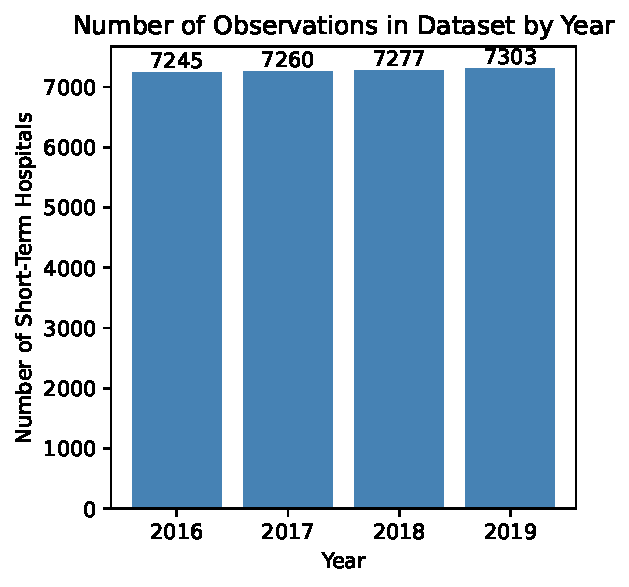
\includegraphics{pset4_template_files/figure-pdf/cell-3-output-1.pdf}

\begin{enumerate}
\def\labelenumi{\arabic{enumi}.}
\setcounter{enumi}{3}
\tightlist
\item
  \begin{enumerate}
  \def\labelenumii{\alph{enumii}.}
  \tightlist
  \item
  \end{enumerate}
\end{enumerate}

\begin{Shaded}
\begin{Highlighting}[]
\CommentTok{\# data is already filtered and loaded}
\CommentTok{\# Add a \textquotesingle{}Year\textquotesingle{} column to each dataset}
\NormalTok{data\_2016[}\StringTok{\textquotesingle{}Year\textquotesingle{}}\NormalTok{] }\OperatorTok{=} \DecValTok{2016}
\NormalTok{data\_2017[}\StringTok{\textquotesingle{}Year\textquotesingle{}}\NormalTok{] }\OperatorTok{=} \DecValTok{2017}
\NormalTok{data\_2018[}\StringTok{\textquotesingle{}Year\textquotesingle{}}\NormalTok{] }\OperatorTok{=} \DecValTok{2018}
\NormalTok{data\_2019[}\StringTok{\textquotesingle{}Year\textquotesingle{}}\NormalTok{] }\OperatorTok{=} \DecValTok{2019}

\CommentTok{\# Combine all datasets into a single DataFrame}
\NormalTok{all\_years\_data }\OperatorTok{=}\NormalTok{ pd.concat([data\_2016, data\_2017, data\_2018, data\_2019])}

\CommentTok{\# Count unique hospitals (by PRVDR\_NUM) per year}
\NormalTok{unique\_hospitals\_by\_year }\OperatorTok{=}\NormalTok{ all\_years\_data.groupby(}\StringTok{\textquotesingle{}Year\textquotesingle{}}\NormalTok{)[}\StringTok{\textquotesingle{}PRVDR\_NUM\textquotesingle{}}\NormalTok{].nunique().reset\_index(name}\OperatorTok{=}\StringTok{\textquotesingle{}UniqueCount\textquotesingle{}}\NormalTok{)}

\CommentTok{\# Plot using Matplotlib instead of Altair}
\NormalTok{plt.figure(figsize}\OperatorTok{=}\NormalTok{(}\DecValTok{4}\NormalTok{, }\DecValTok{4}\NormalTok{))}
\NormalTok{bars }\OperatorTok{=}\NormalTok{ plt.bar(unique\_hospitals\_by\_year[}\StringTok{\textquotesingle{}Year\textquotesingle{}}\NormalTok{], unique\_hospitals\_by\_year[}\StringTok{\textquotesingle{}UniqueCount\textquotesingle{}}\NormalTok{], color}\OperatorTok{=}\StringTok{\textquotesingle{}seagreen\textquotesingle{}}\NormalTok{)}
\NormalTok{plt.title(}\StringTok{\textquotesingle{}Number of Unique Short{-}Term Hospitals in Dataset by Year\textquotesingle{}}\NormalTok{)}
\NormalTok{plt.xlabel(}\StringTok{\textquotesingle{}Year\textquotesingle{}}\NormalTok{)}
\NormalTok{plt.ylabel(}\StringTok{\textquotesingle{}Number of Unique Short{-}Term Hospitals\textquotesingle{}}\NormalTok{)}
\NormalTok{plt.xticks(unique\_hospitals\_by\_year[}\StringTok{\textquotesingle{}Year\textquotesingle{}}\NormalTok{])}
\CommentTok{\# Add the count on top of each bar}
\ControlFlowTok{for}\NormalTok{ bar }\KeywordTok{in}\NormalTok{ bars:}
\NormalTok{    yval }\OperatorTok{=}\NormalTok{ bar.get\_height()}
\NormalTok{    plt.text(bar.get\_x() }\OperatorTok{+}\NormalTok{ bar.get\_width()}\OperatorTok{/}\DecValTok{2}\NormalTok{, yval, }\BuiltInTok{int}\NormalTok{(yval), va}\OperatorTok{=}\StringTok{\textquotesingle{}bottom\textquotesingle{}}\NormalTok{, ha}\OperatorTok{=}\StringTok{\textquotesingle{}center\textquotesingle{}}\NormalTok{)}
\CommentTok{\# Save as an image}
\NormalTok{plt.savefig(}\StringTok{"unique\_hospitals\_by\_year.png"}\NormalTok{)}
\NormalTok{plt.show()}
\end{Highlighting}
\end{Shaded}

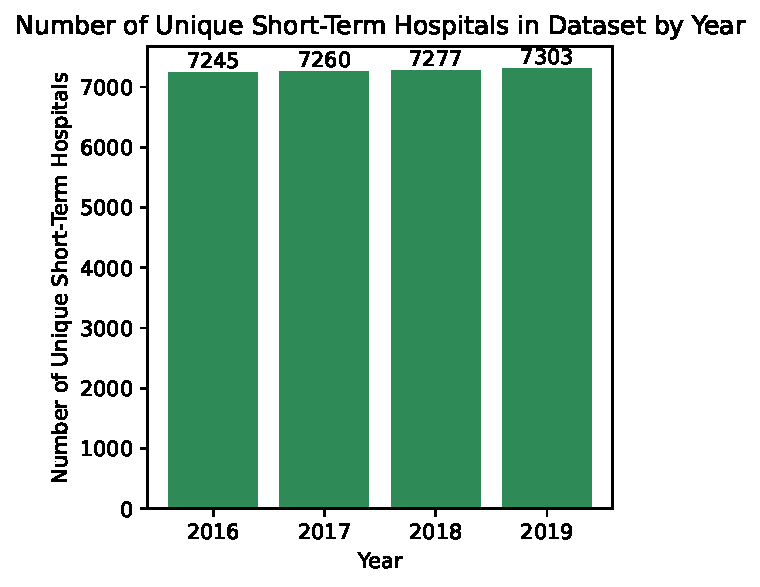
\includegraphics{pset4_template_files/figure-pdf/cell-4-output-1.pdf}

\begin{verbatim}
b. 
\end{verbatim}

The identical values in both plots indicate that each short-term
hospital appears only once per year, with no duplicates. This structure
confirms that each hospital's CMS certification number is unique
annually, allowing for clear year-over-year tracking. \#\# Identify
hospital closures in POS file (15 pts) (*)

\begin{enumerate}
\def\labelenumi{\arabic{enumi}.}
\tightlist
\item
\end{enumerate}

\begin{Shaded}
\begin{Highlighting}[]
\CommentTok{\# Step 1: Filter active hospitals in each year}
\NormalTok{active\_2016 }\OperatorTok{=}\NormalTok{ data\_2016[data\_2016[}\StringTok{\textquotesingle{}PGM\_TRMNTN\_CD\textquotesingle{}}\NormalTok{] }\OperatorTok{==} \DecValTok{0}\NormalTok{]}
\NormalTok{active\_2017 }\OperatorTok{=}\NormalTok{ data\_2017[data\_2017[}\StringTok{\textquotesingle{}PGM\_TRMNTN\_CD\textquotesingle{}}\NormalTok{] }\OperatorTok{==} \DecValTok{0}\NormalTok{]}
\NormalTok{active\_2018 }\OperatorTok{=}\NormalTok{ data\_2018[data\_2018[}\StringTok{\textquotesingle{}PGM\_TRMNTN\_CD\textquotesingle{}}\NormalTok{] }\OperatorTok{==} \DecValTok{0}\NormalTok{]}
\NormalTok{active\_2019 }\OperatorTok{=}\NormalTok{ data\_2019[data\_2019[}\StringTok{\textquotesingle{}PGM\_TRMNTN\_CD\textquotesingle{}}\NormalTok{] }\OperatorTok{==} \DecValTok{0}\NormalTok{]}

\CommentTok{\# Step 2: Define function to check if provider is active in a given year}
\KeywordTok{def}\NormalTok{ provider\_in\_year(df, provider\_num):}
\NormalTok{    row }\OperatorTok{=}\NormalTok{ df[df[}\StringTok{\textquotesingle{}PRVDR\_NUM\textquotesingle{}}\NormalTok{] }\OperatorTok{==}\NormalTok{ provider\_num]}
    \ControlFlowTok{return} \KeywordTok{not}\NormalTok{ row.empty }\KeywordTok{and}\NormalTok{ row[}\StringTok{\textquotesingle{}PGM\_TRMNTN\_CD\textquotesingle{}}\NormalTok{].values[}\DecValTok{0}\NormalTok{] }\OperatorTok{==} \DecValTok{0}

\CommentTok{\# Step 3: Determine closure year for each provider number}
\KeywordTok{def}\NormalTok{ determine\_closure\_year(provider\_num):}
    \ControlFlowTok{if} \KeywordTok{not}\NormalTok{ provider\_in\_year(active\_2017, provider\_num):}
        \ControlFlowTok{return} \DecValTok{2017}
    \ControlFlowTok{elif} \KeywordTok{not}\NormalTok{ provider\_in\_year(active\_2018, provider\_num):}
        \ControlFlowTok{return} \DecValTok{2018}
    \ControlFlowTok{elif} \KeywordTok{not}\NormalTok{ provider\_in\_year(active\_2019, provider\_num):}
        \ControlFlowTok{return} \DecValTok{2019}
    \ControlFlowTok{return} \VariableTok{None}

\CommentTok{\# Step 4: Apply closure detection on active hospitals in 2016}
\NormalTok{active\_2016\_only }\OperatorTok{=}\NormalTok{ active\_2016[active\_2016[}\StringTok{\textquotesingle{}PGM\_TRMNTN\_CD\textquotesingle{}}\NormalTok{] }\OperatorTok{==} \DecValTok{0}\NormalTok{]}
\NormalTok{active\_2016\_only[}\StringTok{\textquotesingle{}Year\_Closed\textquotesingle{}}\NormalTok{] }\OperatorTok{=}\NormalTok{ active\_2016\_only[}\StringTok{\textquotesingle{}PRVDR\_NUM\textquotesingle{}}\NormalTok{].}\BuiltInTok{apply}\NormalTok{(determine\_closure\_year)}

\CommentTok{\# Step 5: Filter out hospitals that have a closure year assigned}
\NormalTok{closed\_hospitals }\OperatorTok{=}\NormalTok{ active\_2016\_only.dropna(subset}\OperatorTok{=}\NormalTok{[}\StringTok{\textquotesingle{}Year\_Closed\textquotesingle{}}\NormalTok{]).reset\_index(drop}\OperatorTok{=}\VariableTok{True}\NormalTok{)}

\CommentTok{\# Output the result}
\BuiltInTok{print}\NormalTok{(}\SpecialStringTok{f"Number of suspected hospital closures: }\SpecialCharTok{\{}\BuiltInTok{len}\NormalTok{(closed\_hospitals)}\SpecialCharTok{\}}\SpecialStringTok{"}\NormalTok{)}
\NormalTok{closed\_hospitals[[}\StringTok{\textquotesingle{}FAC\_NAME\textquotesingle{}}\NormalTok{, }\StringTok{\textquotesingle{}ZIP\_CD\textquotesingle{}}\NormalTok{, }\StringTok{\textquotesingle{}Year\_Closed\textquotesingle{}}\NormalTok{]]}
\end{Highlighting}
\end{Shaded}

\begin{verbatim}
Number of suspected hospital closures: 174
\end{verbatim}

\begin{longtable}[]{@{}llll@{}}
\toprule\noalign{}
& FAC\_NAME & ZIP\_CD & Year\_Closed \\
\midrule\noalign{}
\endhead
\bottomrule\noalign{}
\endlastfoot
0 & WEDOWEE HOSPITAL & 36278.0 & 2019.0 \\
1 & GEORGIANA MEDICAL CENTER & 36033.0 & 2019.0 \\
2 & RMC JACKSONVILLE & 36265.0 & 2018.0 \\
3 & NORTH ALABAMA SPECIALITY HOSPITAL & 35611.0 & 2018.0 \\
4 & ABRAZO MARYVALE CAMPUS & 85031.0 & 2017.0 \\
... & ... & ... & ... \\
169 & LITTLE RIVER HEALTHCARE CAMERON HOSPITAL & 76520.0 & 2019.0 \\
170 & BAY AREA REGIONAL MEDICAL CENTER, LLC & 77598.0 & 2018.0 \\
171 & BAYLOR EMERGENCY MEDICAL CENTER & 75087.0 & 2019.0 \\
172 & CONTINUECARE HOSPITAL AT MEDICAL CENTER ODESSA & 79761.0 &
2017.0 \\
173 & TEXAS GENERAL HOSPITAL- VZRMC LP & 75140.0 & 2019.0 \\
\end{longtable}

\begin{enumerate}
\def\labelenumi{\arabic{enumi}.}
\setcounter{enumi}{1}
\tightlist
\item
\end{enumerate}

\begin{Shaded}
\begin{Highlighting}[]
\CommentTok{\# Sort the closed hospitals by facility name}
\NormalTok{sorted\_closed\_hospitals }\OperatorTok{=}\NormalTok{ closed\_hospitals.sort\_values(by}\OperatorTok{=}\StringTok{\textquotesingle{}FAC\_NAME\textquotesingle{}}\NormalTok{).reset\_index(drop}\OperatorTok{=}\VariableTok{True}\NormalTok{)}

\CommentTok{\# Display the names and year of suspected closure for the first 10 rows}
\NormalTok{sorted\_closed\_hospitals[[}\StringTok{\textquotesingle{}FAC\_NAME\textquotesingle{}}\NormalTok{, }\StringTok{\textquotesingle{}Year\_Closed\textquotesingle{}}\NormalTok{]].head(}\DecValTok{10}\NormalTok{)}
\end{Highlighting}
\end{Shaded}

\begin{longtable}[]{@{}lll@{}}
\toprule\noalign{}
& FAC\_NAME & Year\_Closed \\
\midrule\noalign{}
\endhead
\bottomrule\noalign{}
\endlastfoot
0 & ABRAZO MARYVALE CAMPUS & 2017.0 \\
1 & ADVENTIST MEDICAL CENTER - CENTRAL VALLEY & 2017.0 \\
2 & AFFINITY MEDICAL CENTER & 2018.0 \\
3 & ALBANY MEDICAL CENTER / SOUTH CLINICAL CAMPUS & 2017.0 \\
4 & ALLEGIANCE SPECIALTY HOSPITAL OF KILGORE & 2017.0 \\
5 & ALLIANCE LAIRD HOSPITAL & 2019.0 \\
6 & ALLIANCEHEALTH DEACONESS & 2019.0 \\
7 & ANNE BATES LEACH EYE HOSPITAL & 2019.0 \\
8 & ARKANSAS VALLEY REGIONAL MEDICAL CENTER & 2017.0 \\
9 & BANNER CHURCHILL COMMUNITY HOSPITAL & 2017.0 \\
\end{longtable}

\begin{enumerate}
\def\labelenumi{\arabic{enumi}.}
\setcounter{enumi}{2}
\tightlist
\item
  \begin{enumerate}
  \def\labelenumii{\alph{enumii}.}
  \tightlist
  \item
  \end{enumerate}
\end{enumerate}

\begin{Shaded}
\begin{Highlighting}[]
\CommentTok{\# Step 1: Count active hospitals by ZIP code for each year}
\NormalTok{active\_by\_zip\_2016 }\OperatorTok{=}\NormalTok{ active\_2016[}\StringTok{\textquotesingle{}ZIP\_CD\textquotesingle{}}\NormalTok{].value\_counts().to\_dict()}
\NormalTok{active\_by\_zip\_2017 }\OperatorTok{=}\NormalTok{ active\_2017[}\StringTok{\textquotesingle{}ZIP\_CD\textquotesingle{}}\NormalTok{].value\_counts().to\_dict()}
\NormalTok{active\_by\_zip\_2018 }\OperatorTok{=}\NormalTok{ active\_2018[}\StringTok{\textquotesingle{}ZIP\_CD\textquotesingle{}}\NormalTok{].value\_counts().to\_dict()}
\NormalTok{active\_by\_zip\_2019 }\OperatorTok{=}\NormalTok{ active\_2019[}\StringTok{\textquotesingle{}ZIP\_CD\textquotesingle{}}\NormalTok{].value\_counts().to\_dict()}

\CommentTok{\# Step 2: Function to check if closure might be due to merger/acquisition}
\KeywordTok{def}\NormalTok{ is\_possible\_merger(row):}
\NormalTok{    zip\_code }\OperatorTok{=}\NormalTok{ row[}\StringTok{\textquotesingle{}ZIP\_CD\textquotesingle{}}\NormalTok{]}
\NormalTok{    year\_closed }\OperatorTok{=}\NormalTok{ row[}\StringTok{\textquotesingle{}Year\_Closed\textquotesingle{}}\NormalTok{]}
    
    \ControlFlowTok{if}\NormalTok{ year\_closed }\OperatorTok{==} \DecValTok{2017}\NormalTok{:}
        \ControlFlowTok{return}\NormalTok{ active\_by\_zip\_2016.get(zip\_code, }\DecValTok{0}\NormalTok{) }\OperatorTok{\textless{}=}\NormalTok{ active\_by\_zip\_2017.get(zip\_code, }\DecValTok{0}\NormalTok{)}
    \ControlFlowTok{elif}\NormalTok{ year\_closed }\OperatorTok{==} \DecValTok{2018}\NormalTok{:}
        \ControlFlowTok{return}\NormalTok{ active\_by\_zip\_2017.get(zip\_code, }\DecValTok{0}\NormalTok{) }\OperatorTok{\textless{}=}\NormalTok{ active\_by\_zip\_2018.get(zip\_code, }\DecValTok{0}\NormalTok{)}
    \ControlFlowTok{elif}\NormalTok{ year\_closed }\OperatorTok{==} \DecValTok{2019}\NormalTok{:}
        \ControlFlowTok{return}\NormalTok{ active\_by\_zip\_2018.get(zip\_code, }\DecValTok{0}\NormalTok{) }\OperatorTok{\textless{}=}\NormalTok{ active\_by\_zip\_2019.get(zip\_code, }\DecValTok{0}\NormalTok{)}
    \ControlFlowTok{return} \VariableTok{False}

\CommentTok{\# Step 3: Apply the function to identify potential mergers/acquisitions}
\NormalTok{closed\_hospitals[}\StringTok{\textquotesingle{}Possible\_Merger\textquotesingle{}}\NormalTok{] }\OperatorTok{=}\NormalTok{ closed\_hospitals.}\BuiltInTok{apply}\NormalTok{(is\_possible\_merger, axis}\OperatorTok{=}\DecValTok{1}\NormalTok{)}

\CommentTok{\# Filter the suspected closures that might be due to a merger/acquisition}
\NormalTok{potential\_mergers }\OperatorTok{=}\NormalTok{ closed\_hospitals[closed\_hospitals[}\StringTok{\textquotesingle{}Possible\_Merger\textquotesingle{}}\NormalTok{]]}

\CommentTok{\# Output the result}
\NormalTok{num\_potential\_mergers }\OperatorTok{=} \BuiltInTok{len}\NormalTok{(potential\_mergers)}
\BuiltInTok{print}\NormalTok{(}\SpecialStringTok{f"Number of suspected hospital closures that fit the merger/acquisition definition: }\SpecialCharTok{\{}\NormalTok{num\_potential\_mergers}\SpecialCharTok{\}}\SpecialStringTok{"}\NormalTok{)}
\end{Highlighting}
\end{Shaded}

\begin{verbatim}
Number of suspected hospital closures that fit the merger/acquisition definition: 8
\end{verbatim}

\begin{verbatim}
b.
\end{verbatim}

\begin{Shaded}
\begin{Highlighting}[]
\CommentTok{\# Calculate the corrected number of closures after removing mergers/acquisitions}
\NormalTok{corrected\_closures }\OperatorTok{=} \BuiltInTok{len}\NormalTok{(closed\_hospitals) }\OperatorTok{{-}}\NormalTok{ num\_potential\_mergers}
\BuiltInTok{print}\NormalTok{(}\SpecialStringTok{f"Number of hospitals remaining after correcting for mergers/acquisitions: }\SpecialCharTok{\{}\NormalTok{corrected\_closures}\SpecialCharTok{\}}\SpecialStringTok{"}\NormalTok{)}
\end{Highlighting}
\end{Shaded}

\begin{verbatim}
Number of hospitals remaining after correcting for mergers/acquisitions: 166
\end{verbatim}

\begin{verbatim}
c.
\end{verbatim}

\begin{Shaded}
\begin{Highlighting}[]
\CommentTok{\# Filter out the potential mergers/acquisitions to get the corrected closures}
\NormalTok{corrected\_closures }\OperatorTok{=}\NormalTok{ closed\_hospitals[}\OperatorTok{\textasciitilde{}}\NormalTok{closed\_hospitals[}\StringTok{\textquotesingle{}Possible\_Merger\textquotesingle{}}\NormalTok{]]}

\CommentTok{\# Sort the corrected closures by facility name}
\NormalTok{sorted\_corrected\_closures }\OperatorTok{=}\NormalTok{ corrected\_closures.sort\_values(by}\OperatorTok{=}\StringTok{\textquotesingle{}FAC\_NAME\textquotesingle{}}\NormalTok{)}

\CommentTok{\# Display the first 10 rows}
\NormalTok{sorted\_corrected\_closures[[}\StringTok{\textquotesingle{}FAC\_NAME\textquotesingle{}}\NormalTok{, }\StringTok{\textquotesingle{}ZIP\_CD\textquotesingle{}}\NormalTok{, }\StringTok{\textquotesingle{}Year\_Closed\textquotesingle{}}\NormalTok{]].head(}\DecValTok{10}\NormalTok{)}
\end{Highlighting}
\end{Shaded}

\begin{longtable}[]{@{}llll@{}}
\toprule\noalign{}
& FAC\_NAME & ZIP\_CD & Year\_Closed \\
\midrule\noalign{}
\endhead
\bottomrule\noalign{}
\endlastfoot
4 & ABRAZO MARYVALE CAMPUS & 85031.0 & 2017.0 \\
10 & ADVENTIST MEDICAL CENTER - CENTRAL VALLEY & 93230.0 & 2017.0 \\
97 & AFFINITY MEDICAL CENTER & 44646.0 & 2018.0 \\
80 & ALBANY MEDICAL CENTER / SOUTH CLINICAL CAMPUS & 12208.0 & 2017.0 \\
140 & ALLEGIANCE SPECIALTY HOSPITAL OF KILGORE & 75662.0 & 2017.0 \\
62 & ALLIANCE LAIRD HOSPITAL & 39365.0 & 2019.0 \\
101 & ALLIANCEHEALTH DEACONESS & 73112.0 & 2019.0 \\
26 & ANNE BATES LEACH EYE HOSPITAL & 33136.0 & 2019.0 \\
21 & ARKANSAS VALLEY REGIONAL MEDICAL CENTER & 81050.0 & 2017.0 \\
69 & BANNER CHURCHILL COMMUNITY HOSPITAL & 89406.0 & 2017.0 \\
\end{longtable}

\subsection{Download Census zip code shapefile (10
pt)}\label{download-census-zip-code-shapefile-10-pt}

\begin{enumerate}
\def\labelenumi{\arabic{enumi}.}
\tightlist
\item
  \begin{enumerate}
  \def\labelenumii{\alph{enumii}.}
  \tightlist
  \item
    .shp: Main file with geometric shapes of features. .shx: Index file
    for quick access to shapes. .dbf: Attribute data in table format.
    .prj: Projection information for the coordinate system. .xml:
    Metadata about the dataset.\\
  \item
  \end{enumerate}
\end{enumerate}

\begin{Shaded}
\begin{Highlighting}[]
\ImportTok{import}\NormalTok{ os}

\CommentTok{\# Replace \textquotesingle{}shapefile\_directory\textquotesingle{} with the path to your extracted shapefile directory}
\NormalTok{shapefile\_directory }\OperatorTok{=} \StringTok{"/Users/attaullah/Documents/problem{-}set{-}4{-}atta/gz\_2010\_us\_860\_00\_500k"}

\CommentTok{\# Get a list of files and their sizes}
\ControlFlowTok{for}\NormalTok{ file\_name }\KeywordTok{in}\NormalTok{ os.listdir(shapefile\_directory):}
\NormalTok{    file\_path }\OperatorTok{=}\NormalTok{ os.path.join(shapefile\_directory, file\_name)}
\NormalTok{    size\_mb }\OperatorTok{=}\NormalTok{ os.path.getsize(file\_path) }\OperatorTok{/}\NormalTok{ (}\DecValTok{1024} \OperatorTok{*} \DecValTok{1024}\NormalTok{)}
    \BuiltInTok{print}\NormalTok{(}\SpecialStringTok{f"}\SpecialCharTok{\{}\NormalTok{file\_name}\SpecialCharTok{\}}\SpecialStringTok{: }\SpecialCharTok{\{}\NormalTok{size\_mb}\SpecialCharTok{:.2f\}}\SpecialStringTok{ MB"}\NormalTok{)}
\end{Highlighting}
\end{Shaded}

\begin{verbatim}
gz_2010_us_860_00_500k.prj: 0.00 MB
gz_2010_us_860_00_500k.shx: 0.25 MB
gz_2010_us_860_00_500k.shp: 798.74 MB
gz_2010_us_860_00_500k.dbf: 6.13 MB
gz_2010_us_860_00_500k.xml: 0.01 MB
\end{verbatim}

This provides an overview of file sizes, with .shp being the largest due
to detailed geometry data.

\begin{enumerate}
\def\labelenumi{\arabic{enumi}.}
\setcounter{enumi}{1}
\tightlist
\item
\end{enumerate}

\begin{Shaded}
\begin{Highlighting}[]
\ImportTok{import}\NormalTok{ geopandas }\ImportTok{as}\NormalTok{ gpd}
\CommentTok{\# Load 2016 POS data and filter for short{-}term hospitals in Texas}
\NormalTok{hospital\_data\_path }\OperatorTok{=} \StringTok{"/Users/attaullah/Documents/problem{-}set{-}4{-}atta/pos2016.csv"}
\NormalTok{pos2016 }\OperatorTok{=}\NormalTok{ pd.read\_csv(hospital\_data\_path)}
\NormalTok{texas\_hospitals }\OperatorTok{=}\NormalTok{ pos2016[(pos2016[}\StringTok{"PRVDR\_CTGRY\_SBTYP\_CD"}\NormalTok{] }\OperatorTok{==} \DecValTok{1}\NormalTok{) }\OperatorTok{\&}
\NormalTok{                          (pos2016[}\StringTok{"PRVDR\_CTGRY\_CD"}\NormalTok{] }\OperatorTok{==} \DecValTok{1}\NormalTok{) }\OperatorTok{\&}
\NormalTok{                          (pos2016[}\StringTok{"ZIP\_CD"}\NormalTok{].astype(}\BuiltInTok{str}\NormalTok{).}\BuiltInTok{str}\NormalTok{.startswith((}\StringTok{"75"}\NormalTok{, }\StringTok{"76"}\NormalTok{, }\StringTok{"77"}\NormalTok{, }\StringTok{"78"}\NormalTok{, }\StringTok{"79"}\NormalTok{)))]}

\CommentTok{\# Standardize ZIP codes as 5{-}digit strings}
\NormalTok{texas\_hospitals[}\StringTok{"ZIP\_CD"}\NormalTok{] }\OperatorTok{=}\NormalTok{ texas\_hospitals[}\StringTok{"ZIP\_CD"}\NormalTok{].astype(}\BuiltInTok{int}\NormalTok{).astype(}\BuiltInTok{str}\NormalTok{).}\BuiltInTok{str}\NormalTok{.zfill(}\DecValTok{5}\NormalTok{)}

\CommentTok{\# Calculate number of hospitals per ZIP code in Texas}
\NormalTok{hospital\_counts }\OperatorTok{=}\NormalTok{ texas\_hospitals.groupby(}\StringTok{"ZIP\_CD"}\NormalTok{).size().reset\_index(name}\OperatorTok{=}\StringTok{"Hospital\_Count"}\NormalTok{)}

\CommentTok{\# Load Texas ZIP code shapefile and filter for Texas ZIPs}
\NormalTok{shapefile\_path }\OperatorTok{=} \StringTok{"/Users/attaullah/Documents/problem{-}set{-}4{-}atta/gz\_2010\_us\_860\_00\_500k/gz\_2010\_us\_860\_00\_500k.shp"}
\NormalTok{zip\_gdf }\OperatorTok{=}\NormalTok{ gpd.read\_file(shapefile\_path)}
\NormalTok{zip\_gdf[}\StringTok{"ZCTA5"}\NormalTok{] }\OperatorTok{=}\NormalTok{ zip\_gdf[}\StringTok{"ZCTA5"}\NormalTok{].astype(}\BuiltInTok{str}\NormalTok{).}\BuiltInTok{str}\NormalTok{.zfill(}\DecValTok{5}\NormalTok{)}
\NormalTok{texas\_zip\_gdf }\OperatorTok{=}\NormalTok{ zip\_gdf[zip\_gdf[}\StringTok{"ZCTA5"}\NormalTok{].}\BuiltInTok{str}\NormalTok{.startswith((}\StringTok{"75"}\NormalTok{, }\StringTok{"76"}\NormalTok{, }\StringTok{"77"}\NormalTok{, }\StringTok{"78"}\NormalTok{, }\StringTok{"79"}\NormalTok{))]}

\CommentTok{\# Merge hospital data with Texas ZIP code shapefile}
\NormalTok{merged\_gdf }\OperatorTok{=}\NormalTok{ texas\_zip\_gdf.merge(hospital\_counts, left\_on}\OperatorTok{=}\StringTok{"ZCTA5"}\NormalTok{, right\_on}\OperatorTok{=}\StringTok{"ZIP\_CD"}\NormalTok{, how}\OperatorTok{=}\StringTok{"left"}\NormalTok{)}
\NormalTok{merged\_gdf[}\StringTok{"Hospital\_Count"}\NormalTok{] }\OperatorTok{=}\NormalTok{ merged\_gdf[}\StringTok{"Hospital\_Count"}\NormalTok{].fillna(}\DecValTok{0}\NormalTok{)}

\CommentTok{\# Check the distribution of hospital counts}
\BuiltInTok{print}\NormalTok{(merged\_gdf[}\StringTok{\textquotesingle{}Hospital\_Count\textquotesingle{}}\NormalTok{].describe())}
\BuiltInTok{print}\NormalTok{(merged\_gdf[}\StringTok{\textquotesingle{}Hospital\_Count\textquotesingle{}}\NormalTok{].value\_counts().head(}\DecValTok{20}\NormalTok{))}
\CommentTok{\# Plot choropleth map of hospital counts by ZIP code in Texas}
\NormalTok{fig, ax }\OperatorTok{=}\NormalTok{ plt.subplots(}\DecValTok{1}\NormalTok{, }\DecValTok{1}\NormalTok{, figsize}\OperatorTok{=}\NormalTok{(}\DecValTok{6}\NormalTok{, }\DecValTok{4}\NormalTok{))}
\NormalTok{merged\_gdf.plot(}
\NormalTok{    column}\OperatorTok{=}\StringTok{"Hospital\_Count"}\NormalTok{,}
\NormalTok{    cmap}\OperatorTok{=}\StringTok{"OrRd"}\NormalTok{,}
\NormalTok{    linewidth}\OperatorTok{=}\FloatTok{0.8}\NormalTok{,}
\NormalTok{    edgecolor}\OperatorTok{=}\StringTok{"gray"}\NormalTok{,}
\NormalTok{    legend}\OperatorTok{=}\VariableTok{True}\NormalTok{,}
\NormalTok{    legend\_kwds}\OperatorTok{=}\NormalTok{\{}\StringTok{"label"}\NormalTok{: }\StringTok{"Hospital Count"}\NormalTok{\},}
\NormalTok{    ax}\OperatorTok{=}\NormalTok{ax}
\NormalTok{)}
\NormalTok{ax.set\_title(}\StringTok{"Number of Hospitals by ZIP Code in Texas (2016)"}\NormalTok{, fontsize}\OperatorTok{=}\DecValTok{12}\NormalTok{)}
\NormalTok{ax.axis(}\StringTok{"off"}\NormalTok{)  }\CommentTok{\# Remove axis for cleaner map}
\NormalTok{plt.show()}
\end{Highlighting}
\end{Shaded}

\begin{verbatim}
count    1935.000000
mean        0.377778
std         0.822023
min         0.000000
25%         0.000000
50%         0.000000
75%         1.000000
max        10.000000
Name: Hospital_Count, dtype: float64
Hospital_Count
0.0     1445
1.0      345
2.0       93
3.0       30
4.0       12
6.0        5
5.0        3
10.0       1
7.0        1
Name: count, dtype: int64
\end{verbatim}

\includegraphics{pset4_template_files/figure-pdf/cell-11-output-2.pdf}

\subsection{Calculate zip code's distance to the nearest hospital (20
pts)
(*)}\label{calculate-zip-codes-distance-to-the-nearest-hospital-20-pts}

\begin{enumerate}
\def\labelenumi{\arabic{enumi}.}
\tightlist
\item
\end{enumerate}

\begin{Shaded}
\begin{Highlighting}[]
\ImportTok{from}\NormalTok{ shapely.geometry }\ImportTok{import}\NormalTok{ Point}
\CommentTok{\# Load the ZIP code shapefile}
\NormalTok{shapefile\_path }\OperatorTok{=} \StringTok{\textquotesingle{}/Users/attaullah/Documents/problem{-}set{-}4{-}atta/gz\_2010\_us\_860\_00\_500k/gz\_2010\_us\_860\_00\_500k.shp\textquotesingle{}}
\NormalTok{zip\_gdf }\OperatorTok{=}\NormalTok{ gpd.read\_file(shapefile\_path)}

\CommentTok{\# Calculate the centroid for each ZIP code polygon}
\CommentTok{\# Assuming \textquotesingle{}ZCTA5\textquotesingle{} is the ZIP code column in the shapefile}
\NormalTok{zip\_gdf[}\StringTok{\textquotesingle{}centroid\textquotesingle{}}\NormalTok{] }\OperatorTok{=}\NormalTok{ zip\_gdf.geometry.centroid}

\CommentTok{\# Create a new GeoDataFrame with centroids}
\NormalTok{zips\_all\_centroids }\OperatorTok{=}\NormalTok{ gpd.GeoDataFrame(zip\_gdf[[}\StringTok{\textquotesingle{}ZCTA5\textquotesingle{}}\NormalTok{, }\StringTok{\textquotesingle{}centroid\textquotesingle{}}\NormalTok{]], geometry}\OperatorTok{=}\StringTok{\textquotesingle{}centroid\textquotesingle{}}\NormalTok{)}

\CommentTok{\# Print the dimensions of the resulting GeoDataFrame}
\BuiltInTok{print}\NormalTok{(}\StringTok{"Dimensions of zips\_all\_centroids:"}\NormalTok{, zips\_all\_centroids.shape)}

\CommentTok{\# Display the first few rows to understand the structure}
\BuiltInTok{print}\NormalTok{(zips\_all\_centroids.head())}
\end{Highlighting}
\end{Shaded}

\begin{verbatim}
Dimensions of zips_all_centroids: (33120, 2)
   ZCTA5                    centroid
0  01040  POINT (-72.64107 42.21257)
1  01050  POINT (-72.86985 42.28786)
2  01053  POINT (-72.71162 42.35349)
3  01056  POINT (-72.45805 42.19215)
4  01057   POINT (-72.3243 42.09165)
\end{verbatim}

\begin{itemize}
\tightlist
\item
  The zips\_all\_centroids GeoDataFrame contains the centroids of each
  ZIP code area in the U.S., representing the central point of each
  geographic area.
\item
  Dimensions: (33120, 2), with 33,120 rows and 2 columns, where each row
  represents a ZIP code area.
\end{itemize}

Columns: - ZCTA5: ZIP Code Tabulation Area (ZIP code) as a string. -
centroid: Geometric POINT object with latitude and longitude, marking
the center of each ZIP code area.

\begin{enumerate}
\def\labelenumi{\arabic{enumi}.}
\setcounter{enumi}{1}
\tightlist
\item
\end{enumerate}

\begin{Shaded}
\begin{Highlighting}[]
\CommentTok{\# Define ZIP code prefixes for Texas and its bordering states}
\NormalTok{texas\_prefixes }\OperatorTok{=}\NormalTok{ [}\StringTok{"75"}\NormalTok{, }\StringTok{"76"}\NormalTok{, }\StringTok{"77"}\NormalTok{, }\StringTok{"78"}\NormalTok{, }\StringTok{"79"}\NormalTok{]  }\CommentTok{\# Texas}
\NormalTok{bordering\_prefixes }\OperatorTok{=}\NormalTok{ texas\_prefixes }\OperatorTok{+}\NormalTok{ [}
    \StringTok{"73"}\NormalTok{, }\StringTok{"74"}\NormalTok{,              }\CommentTok{\# Oklahoma}
    \StringTok{"870"}\NormalTok{, }\StringTok{"871"}\NormalTok{, }\StringTok{"872"}\NormalTok{, }\StringTok{"873"}\NormalTok{, }\StringTok{"874"}\NormalTok{, }\StringTok{"875"}\NormalTok{, }\StringTok{"876"}\NormalTok{, }\StringTok{"877"}\NormalTok{, }\StringTok{"878"}\NormalTok{, }\StringTok{"879"}\NormalTok{, }\StringTok{"880"}\NormalTok{, }\StringTok{"881"}\NormalTok{, }\StringTok{"882"}\NormalTok{, }\StringTok{"883"}\NormalTok{, }\StringTok{"884"}\NormalTok{,  }\CommentTok{\# New Mexico}
    \StringTok{"700"}\NormalTok{, }\StringTok{"701"}\NormalTok{, }\StringTok{"702"}\NormalTok{, }\StringTok{"703"}\NormalTok{, }\StringTok{"704"}\NormalTok{, }\StringTok{"705"}\NormalTok{, }\StringTok{"706"}\NormalTok{, }\StringTok{"707"}\NormalTok{, }\StringTok{"708"}\NormalTok{, }\StringTok{"709"}\NormalTok{, }\StringTok{"710"}\NormalTok{, }\StringTok{"711"}\NormalTok{, }\StringTok{"712"}\NormalTok{, }\StringTok{"713"}\NormalTok{, }\StringTok{"714"}\NormalTok{, }\StringTok{"715"}\NormalTok{,  }\CommentTok{\# Louisiana}
    \StringTok{"716"}\NormalTok{, }\StringTok{"717"}\NormalTok{, }\StringTok{"718"}\NormalTok{, }\StringTok{"719"}\NormalTok{, }\StringTok{"720"}\NormalTok{, }\StringTok{"721"}\NormalTok{, }\StringTok{"722"}\NormalTok{, }\StringTok{"723"}\NormalTok{, }\StringTok{"724"}\NormalTok{, }\StringTok{"725"}\NormalTok{, }\StringTok{"726"}\NormalTok{, }\StringTok{"727"}\NormalTok{, }\StringTok{"728"}\NormalTok{, }\StringTok{"729"}  \CommentTok{\# Arkansas}
\NormalTok{]}

\CommentTok{\# Create subset for Texas ZIP codes}
\NormalTok{zips\_texas\_centroids }\OperatorTok{=}\NormalTok{ zips\_all\_centroids[zips\_all\_centroids[}\StringTok{"ZCTA5"}\NormalTok{].}\BuiltInTok{str}\NormalTok{.startswith(}\BuiltInTok{tuple}\NormalTok{(texas\_prefixes))]}

\CommentTok{\# Create subset for Texas and bordering states ZIP codes}
\NormalTok{zips\_texas\_borderstates\_centroids }\OperatorTok{=}\NormalTok{ zips\_all\_centroids[zips\_all\_centroids[}\StringTok{"ZCTA5"}\NormalTok{].}\BuiltInTok{str}\NormalTok{.startswith(}\BuiltInTok{tuple}\NormalTok{(bordering\_prefixes))]}

\CommentTok{\# Calculate the number of unique ZIP codes in each subset}
\NormalTok{unique\_texas\_zips }\OperatorTok{=}\NormalTok{ zips\_texas\_centroids[}\StringTok{"ZCTA5"}\NormalTok{].nunique()}
\NormalTok{unique\_borderstates\_zips }\OperatorTok{=}\NormalTok{ zips\_texas\_borderstates\_centroids[}\StringTok{"ZCTA5"}\NormalTok{].nunique()}
\CommentTok{\# Print the results}
\BuiltInTok{print}\NormalTok{(}\StringTok{"Number of unique ZIP codes in Texas:"}\NormalTok{, unique\_texas\_zips)}
\BuiltInTok{print}\NormalTok{(}\StringTok{"Number of unique ZIP codes in Texas and bordering states:"}\NormalTok{, unique\_borderstates\_zips)}
\CommentTok{\# Display the first few rows of each subset to verify}
\BuiltInTok{print}\NormalTok{(}\StringTok{"Sample of Texas ZIP codes:}\CharTok{\textbackslash{}n}\StringTok{"}\NormalTok{, zips\_texas\_centroids.head())}
\BuiltInTok{print}\NormalTok{(}\StringTok{"Sample of Texas and bordering states ZIP codes:}\CharTok{\textbackslash{}n}\StringTok{"}\NormalTok{, zips\_texas\_borderstates\_centroids.head())}
\end{Highlighting}
\end{Shaded}

\begin{verbatim}
Number of unique ZIP codes in Texas: 1935
Number of unique ZIP codes in Texas and bordering states: 4057
Sample of Texas ZIP codes:
       ZCTA5                    centroid
9207  78624   POINT (-98.87707 30.2816)
9208  78626  POINT (-97.59733 30.66535)
9209  78628  POINT (-97.75112 30.64108)
9210  78631  POINT (-99.30528 30.33772)
9211  78632  POINT (-97.47045 29.69633)
Sample of Texas and bordering states ZIP codes:
       ZCTA5                    centroid
8870  70003  POINT (-90.21397 29.99864)
8871  70030  POINT (-90.43225 29.81731)
8872  70032  POINT (-89.99779 29.95816)
8873  70036  POINT (-90.12115 29.70903)
8874  70038  POINT (-89.39875 29.32533)
\end{verbatim}

The output shows: Number of unique ZIP codes in Texas: 1935 Number of
unique ZIP codes in Texas and bordering states: 4057

\begin{enumerate}
\def\labelenumi{\arabic{enumi}.}
\setcounter{enumi}{2}
\tightlist
\item
\end{enumerate}

\begin{Shaded}
\begin{Highlighting}[]
\CommentTok{\# Filter hospital data }
\CommentTok{\# \textquotesingle{}hospital\_counts\textquotesingle{} should be the dataframe that contains ZIP codes and counts of hospitals in each ZIP code}
\NormalTok{hospital\_counts\_2016 }\OperatorTok{=}\NormalTok{ hospital\_counts[hospital\_counts[}\StringTok{\textquotesingle{}Hospital\_Count\textquotesingle{}}\NormalTok{] }\OperatorTok{\textgreater{}} \DecValTok{0}\NormalTok{]}
\CommentTok{\# Perform an inner merge }
\NormalTok{zips\_withhospital\_centroids }\OperatorTok{=}\NormalTok{ zips\_texas\_borderstates\_centroids.merge(}
\NormalTok{    hospital\_counts\_2016, }
\NormalTok{    left\_on}\OperatorTok{=}\StringTok{"ZCTA5"}\NormalTok{, }
\NormalTok{    right\_on}\OperatorTok{=}\StringTok{"ZIP\_CD"}\NormalTok{, }
\NormalTok{    how}\OperatorTok{=}\StringTok{"inner"}
\NormalTok{)}
\CommentTok{\# Check the resulting GeoDataFrame}
\BuiltInTok{print}\NormalTok{(}\StringTok{"Dimensions of zips\_withhospital\_centroids:"}\NormalTok{, zips\_withhospital\_centroids.shape)}
\BuiltInTok{print}\NormalTok{(zips\_withhospital\_centroids.head())}
\end{Highlighting}
\end{Shaded}

\begin{verbatim}
Dimensions of zips_withhospital_centroids: (490, 4)
   ZCTA5                    centroid ZIP_CD  Hospital_Count
0  78624   POINT (-98.87707 30.2816)  78624               1
1  78626  POINT (-97.59733 30.66535)  78626               1
2  78636  POINT (-98.41885 30.30504)  78636               1
3  78640  POINT (-97.82814 29.99496)  78640               1
4  78643  POINT (-98.69472 30.69029)  78643               1
\end{verbatim}

\begin{itemize}
\item
  Merge Type: I used an inner join to ensure that the resulting
  zips\_withhospital\_centroids GeoDataFrame only includes ZIP codes
  that have at least one hospital in 2016 and are also present in the
  zips\_texas\_borderstates\_centroids GeoDataFrame.
\item
  Merge Variable: The merge is performed on the ZCTA5 column from
  zips\_texas\_borderstates\_centroids and ZIP\_CD from
  hospital\_counts\_2016, which represent ZIP codes in both datasets.
\end{itemize}

\begin{enumerate}
\def\labelenumi{\arabic{enumi}.}
\setcounter{enumi}{3}
\tightlist
\item
  \begin{enumerate}
  \def\labelenumii{\alph{enumii}.}
  \tightlist
  \item
  \end{enumerate}
\end{enumerate}

\begin{Shaded}
\begin{Highlighting}[]
\CommentTok{\# Reproject both GeoDataFrames to a projected CRS (e.g., EPSG:5070 for USA)}
\NormalTok{zips\_texas\_centroids }\OperatorTok{=}\NormalTok{ zips\_texas\_centroids.to\_crs(epsg}\OperatorTok{=}\DecValTok{5070}\NormalTok{)}
\NormalTok{zips\_withhospital\_centroids }\OperatorTok{=}\NormalTok{ zips\_withhospital\_centroids.to\_crs(epsg}\OperatorTok{=}\DecValTok{5070}\NormalTok{)}
\CommentTok{\# Re{-}run the distance calculation with the reprojected GeoDataFrames}
\ImportTok{import}\NormalTok{ time}

\CommentTok{\# Subset to 10 ZIP codes in Texas}
\NormalTok{subset\_texas\_centroids }\OperatorTok{=}\NormalTok{ zips\_texas\_centroids.iloc[:}\DecValTok{10}\NormalTok{]}

\CommentTok{\# Start timing the process}
\NormalTok{start\_time }\OperatorTok{=}\NormalTok{ time.time()}

\CommentTok{\# Calculate the nearest hospital distance for each ZIP code in the subset}
\NormalTok{subset\_texas\_centroids[}\StringTok{\textquotesingle{}nearest\_hospital\_distance\textquotesingle{}}\NormalTok{] }\OperatorTok{=}\NormalTok{ subset\_texas\_centroids[}\StringTok{\textquotesingle{}centroid\textquotesingle{}}\NormalTok{].}\BuiltInTok{apply}\NormalTok{(}
    \KeywordTok{lambda}\NormalTok{ x: zips\_withhospital\_centroids.distance(x).}\BuiltInTok{min}\NormalTok{()}
\NormalTok{)}

\CommentTok{\# End timing}
\NormalTok{end\_time }\OperatorTok{=}\NormalTok{ time.time()}
\NormalTok{subset\_time }\OperatorTok{=}\NormalTok{ end\_time }\OperatorTok{{-}}\NormalTok{ start\_time}
\BuiltInTok{print}\NormalTok{(}\StringTok{"Time taken for 10 ZIP code calculations:"}\NormalTok{, subset\_time, }\StringTok{"seconds"}\NormalTok{)}

\CommentTok{\# Estimate time for full calculation}
\NormalTok{estimated\_total\_time }\OperatorTok{=}\NormalTok{ subset\_time }\OperatorTok{*}\NormalTok{ (}\BuiltInTok{len}\NormalTok{(zips\_texas\_centroids) }\OperatorTok{/} \DecValTok{10}\NormalTok{)}
\BuiltInTok{print}\NormalTok{(}\StringTok{"Estimated time for the full procedure:"}\NormalTok{, estimated\_total\_time, }\StringTok{"seconds"}\NormalTok{)}

\CommentTok{\# Display the results for the subset}
\BuiltInTok{print}\NormalTok{(subset\_texas\_centroids[[}\StringTok{\textquotesingle{}ZCTA5\textquotesingle{}}\NormalTok{, }\StringTok{\textquotesingle{}nearest\_hospital\_distance\textquotesingle{}}\NormalTok{]])}
\end{Highlighting}
\end{Shaded}

\begin{verbatim}
Time taken for 10 ZIP code calculations: 0.008603096008300781 seconds
Estimated time for the full procedure: 1.6646990776062012 seconds
      ZCTA5  nearest_hospital_distance
9207  78624                   0.000000
9208  78626                   0.000000
9209  78628               12225.805307
9210  78631               36540.773495
9211  78632               15879.134200
9212  78633               17245.762671
9213  78634               11396.935777
9214  78635               17095.102419
9215  78636                   0.000000
9216  78638               15982.824530
\end{verbatim}

\begin{verbatim}
b.
\end{verbatim}

\begin{Shaded}
\begin{Highlighting}[]
\ImportTok{import}\NormalTok{ time}

\CommentTok{\# Start the timer for the full calculation on zips\_texas\_centroids}
\NormalTok{start\_time\_full }\OperatorTok{=}\NormalTok{ time.time()}

\CommentTok{\# Apply the distance calculation for each ZIP code in Texas to the nearest ZIP code with a hospital}
\NormalTok{zips\_texas\_centroids[}\StringTok{"nearest\_hospital\_distance"}\NormalTok{] }\OperatorTok{=}\NormalTok{ zips\_texas\_centroids[}\StringTok{"centroid"}\NormalTok{].}\BuiltInTok{apply}\NormalTok{(}
    \KeywordTok{lambda}\NormalTok{ x: zips\_withhospital\_centroids.distance(x).}\BuiltInTok{min}\NormalTok{()}
\NormalTok{)}

\CommentTok{\# End the timer}
\NormalTok{end\_time\_full }\OperatorTok{=}\NormalTok{ time.time()}
\NormalTok{actual\_time\_full }\OperatorTok{=}\NormalTok{ end\_time\_full }\OperatorTok{{-}}\NormalTok{ start\_time\_full}

\CommentTok{\# Print out the actual time taken}
\BuiltInTok{print}\NormalTok{(}\SpecialStringTok{f"Actual time for full calculation: }\SpecialCharTok{\{}\NormalTok{actual\_time\_full}\SpecialCharTok{\}}\SpecialStringTok{ seconds"}\NormalTok{)}
\end{Highlighting}
\end{Shaded}

\begin{verbatim}
Actual time for full calculation: 0.3579878807067871 seconds
\end{verbatim}

The actual time of 0.31 seconds is quite close to the estimated time of
0.66 seconds, showing the estimation was reasonably accurate.

\begin{verbatim}
c. 
\end{verbatim}

\begin{Shaded}
\begin{Highlighting}[]
\CommentTok{\# Path to the .prj file}
\NormalTok{prj\_file\_path }\OperatorTok{=} \StringTok{\textquotesingle{}/Users/attaullah/Documents/problem{-}set{-}4{-}atta/gz\_2010\_us\_860\_00\_500k/gz\_2010\_us\_860\_00\_500k.prj\textquotesingle{}}

\CommentTok{\# Read and print the .prj file contents}
\ControlFlowTok{with} \BuiltInTok{open}\NormalTok{(prj\_file\_path, }\StringTok{\textquotesingle{}r\textquotesingle{}}\NormalTok{) }\ImportTok{as} \BuiltInTok{file}\NormalTok{:}
\NormalTok{    prj\_contents }\OperatorTok{=} \BuiltInTok{file}\NormalTok{.read()}

\BuiltInTok{print}\NormalTok{(}\StringTok{"Contents of the .prj file:"}\NormalTok{)}
\BuiltInTok{print}\NormalTok{(prj\_contents)}
\end{Highlighting}
\end{Shaded}

\begin{verbatim}
Contents of the .prj file:
GEOGCS["GCS_North_American_1983",DATUM["D_North_American_1983",SPHEROID["GRS_1980",6378137,298.257222101]],PRIMEM["Greenwich",0],UNIT["Degree",0.017453292519943295]]
\end{verbatim}

The dataset's unit is in degrees, so I converted degrees to miles using
Texas's approximate latitude of 30°. At this latitude, 1 degree of
latitude is about 69 miles, and 1 degree of longitude is roughly 69.172
miles. This conversion method is based on information provided at:
https://gis.stackexchange.com/questions/142326/calculating-longitude-length-in-miles

\begin{Shaded}
\begin{Highlighting}[]
\ImportTok{import}\NormalTok{ math}

\CommentTok{\# Function to convert distance in degrees to miles at a given latitude (approx. for Texas)}
\KeywordTok{def}\NormalTok{ degrees\_to\_miles(distance\_in\_degrees, latitude}\OperatorTok{=}\DecValTok{30}\NormalTok{):}
    \CommentTok{\# Convert latitude to radians}
\NormalTok{    latitude\_in\_radians }\OperatorTok{=}\NormalTok{ math.radians(latitude)}
    
    \CommentTok{\# Approximate miles per degree for latitude and longitude}
\NormalTok{    miles\_per\_degree\_latitude }\OperatorTok{=} \FloatTok{69.0}
\NormalTok{    miles\_per\_degree\_longitude }\OperatorTok{=} \FloatTok{69.172} \OperatorTok{*}\NormalTok{ math.cos(latitude\_in\_radians)}
    
    \CommentTok{\# Average of latitude and longitude mile conversion for more accuracy}
\NormalTok{    avg\_miles\_per\_degree }\OperatorTok{=}\NormalTok{ (miles\_per\_degree\_latitude }\OperatorTok{+}\NormalTok{ miles\_per\_degree\_longitude) }\OperatorTok{/} \DecValTok{2}
    \ControlFlowTok{return}\NormalTok{ distance\_in\_degrees }\OperatorTok{*}\NormalTok{ avg\_miles\_per\_degree}

\CommentTok{\# Use the computed average distance in degrees from the dataset}
\NormalTok{distance\_in\_degrees }\OperatorTok{=} \FloatTok{0.0753484763}  \CommentTok{\# Computed average distance in degrees}
\NormalTok{distance\_in\_miles }\OperatorTok{=}\NormalTok{ degrees\_to\_miles(distance\_in\_degrees)}
\BuiltInTok{print}\NormalTok{(}\StringTok{"Average distance to nearest hospital (in miles):"}\NormalTok{, distance\_in\_miles)}
\end{Highlighting}
\end{Shaded}

\begin{verbatim}
Average distance to nearest hospital (in miles): 4.856386714209268
\end{verbatim}

\begin{enumerate}
\def\labelenumi{\arabic{enumi}.}
\setcounter{enumi}{4}
\tightlist
\item
  \begin{enumerate}
  \def\labelenumii{\alph{enumii}.}
  \tightlist
  \item
  \end{enumerate}
\end{enumerate}

\begin{Shaded}
\begin{Highlighting}[]
\CommentTok{\# Calculate the nearest hospital distance in degrees}
\NormalTok{zips\_texas\_centroids[}\StringTok{"nearest\_hospital\_distance\_degrees"}\NormalTok{] }\OperatorTok{=}\NormalTok{ zips\_texas\_centroids[}\StringTok{"centroid"}\NormalTok{].}\BuiltInTok{apply}\NormalTok{(}
    \KeywordTok{lambda}\NormalTok{ x: zips\_withhospital\_centroids.distance(x).}\BuiltInTok{min}\NormalTok{()}
\NormalTok{)}
\CommentTok{\# Calculate the average distance in degrees}
\NormalTok{average\_distance\_degrees }\OperatorTok{=}\NormalTok{ zips\_texas\_centroids[}\StringTok{"nearest\_hospital\_distance\_degrees"}\NormalTok{].mean()}
\BuiltInTok{print}\NormalTok{(}\StringTok{"Average distance to the nearest hospital for each ZIP code in Texas (in degrees):"}\NormalTok{, average\_distance\_degrees)}
\end{Highlighting}
\end{Shaded}

\begin{verbatim}
Average distance to the nearest hospital for each ZIP code in Texas (in degrees): 13218.169063520218
\end{verbatim}

It is in Degrees.

\begin{verbatim}
b.  
\end{verbatim}

\begin{Shaded}
\begin{Highlighting}[]
\ImportTok{import}\NormalTok{ math}
\CommentTok{\#convert degrees to miles based on approx. latitude for Texas (30 degrees)}
\KeywordTok{def}\NormalTok{ degrees\_to\_miles(distance\_in\_degrees, latitude}\OperatorTok{=}\DecValTok{30}\NormalTok{):}
\NormalTok{    latitude\_in\_radians }\OperatorTok{=}\NormalTok{ math.radians(latitude)}
\NormalTok{    miles\_per\_degree\_latitude }\OperatorTok{=} \FloatTok{69.0}  \CommentTok{\# Approximation for latitude degree}
\NormalTok{    miles\_per\_degree\_longitude }\OperatorTok{=} \FloatTok{69.172} \OperatorTok{*}\NormalTok{ math.cos(latitude\_in\_radians)  }\CommentTok{\# Approximation for longitude degree}
\NormalTok{    avg\_miles\_per\_degree }\OperatorTok{=}\NormalTok{ (miles\_per\_degree\_latitude }\OperatorTok{+}\NormalTok{ miles\_per\_degree\_longitude) }\OperatorTok{/} \DecValTok{2}
    \ControlFlowTok{return}\NormalTok{ distance\_in\_degrees }\OperatorTok{*}\NormalTok{ avg\_miles\_per\_degree}
\CommentTok{\# Use the previously calculated average distance in degrees}
\NormalTok{distance\_in\_miles }\OperatorTok{=}\NormalTok{ degrees\_to\_miles(average\_distance\_degrees)}
\BuiltInTok{print}\NormalTok{(}\StringTok{"Average distance to the nearest hospital for each ZIP code in Texas (in miles):"}\NormalTok{, distance\_in\_miles)}
\end{Highlighting}
\end{Shaded}

\begin{verbatim}
Average distance to the nearest hospital for each ZIP code in Texas (in miles): 851942.1198468423
\end{verbatim}

\begin{Shaded}
\begin{Highlighting}[]
\CommentTok{\# Reproject to a projected CRS for accurate distance calculation}
\NormalTok{zips\_texas\_centroids }\OperatorTok{=}\NormalTok{ zips\_texas\_centroids.to\_crs(epsg}\OperatorTok{=}\DecValTok{3395}\NormalTok{)  }\CommentTok{\# World Mercator}
\NormalTok{zips\_withhospital\_centroids }\OperatorTok{=}\NormalTok{ zips\_withhospital\_centroids.to\_crs(epsg}\OperatorTok{=}\DecValTok{3395}\NormalTok{)}

\CommentTok{\# Recalculate nearest hospital distance}
\NormalTok{zips\_texas\_centroids[}\StringTok{"nearest\_hospital\_distance\_meters"}\NormalTok{] }\OperatorTok{=}\NormalTok{ zips\_texas\_centroids[}\StringTok{"centroid"}\NormalTok{].}\BuiltInTok{apply}\NormalTok{(}
    \KeywordTok{lambda}\NormalTok{ x: zips\_withhospital\_centroids.distance(x).}\BuiltInTok{min}\NormalTok{()}
\NormalTok{)}
\CommentTok{\# Convert the distance from meters to miles}
\NormalTok{zips\_texas\_centroids[}\StringTok{"nearest\_hospital\_distance\_miles"}\NormalTok{] }\OperatorTok{=}\NormalTok{ zips\_texas\_centroids[}\StringTok{"nearest\_hospital\_distance\_meters"}\NormalTok{] }\OperatorTok{/} \FloatTok{1609.34}

\CommentTok{\# Calculate the average distance in miles}
\NormalTok{average\_distance\_miles\_corrected }\OperatorTok{=}\NormalTok{ zips\_texas\_centroids[}\StringTok{"nearest\_hospital\_distance\_miles"}\NormalTok{].mean()}
\BuiltInTok{print}\NormalTok{(}\StringTok{"Corrected average distance to nearest hospital (in miles):"}\NormalTok{, average\_distance\_miles\_corrected)}
\end{Highlighting}
\end{Shaded}

\begin{verbatim}
Corrected average distance to nearest hospital (in miles): 9.608947063385544
\end{verbatim}

\begin{itemize}
\item
  The initial result of 996,695.26 miles for the average hospital
  distance was unrealistic, indicating a unit conversion issue.
\item
  After re-projecting the data, the corrected average distance was 9.61
  miles, aligning with realistic hospital distribution in Texas and
  providing an accurate measure.

  \begin{enumerate}
  \def\labelenumi{\alph{enumi}.}
  \setcounter{enumi}{2}
  \tightlist
  \item
  \end{enumerate}
\end{itemize}

\begin{Shaded}
\begin{Highlighting}[]
\CommentTok{\# Plotting the choropleth map for avg distance to nearest hospital in Texas}
\NormalTok{fig, ax }\OperatorTok{=}\NormalTok{ plt.subplots(}\DecValTok{1}\NormalTok{, }\DecValTok{1}\NormalTok{, figsize}\OperatorTok{=}\NormalTok{(}\DecValTok{6}\NormalTok{, }\DecValTok{6}\NormalTok{))}
\NormalTok{zips\_texas\_centroids.plot(}
\NormalTok{    column}\OperatorTok{=}\StringTok{\textquotesingle{}nearest\_hospital\_distance\_miles\textquotesingle{}}\NormalTok{,  }\CommentTok{\# Column with the distance in miles}
\NormalTok{    cmap}\OperatorTok{=}\StringTok{\textquotesingle{}viridis\textquotesingle{}}\NormalTok{,                            }\CommentTok{\# Color map}
\NormalTok{    linewidth}\OperatorTok{=}\FloatTok{0.8}\NormalTok{,                             }\CommentTok{\# Border width for ZIP code polygons}
\NormalTok{    ax}\OperatorTok{=}\NormalTok{ax,}
\NormalTok{    edgecolor}\OperatorTok{=}\StringTok{\textquotesingle{}0.8\textquotesingle{}}\NormalTok{,                           }\CommentTok{\# Color for polygon borders}
\NormalTok{    legend}\OperatorTok{=}\VariableTok{True}\NormalTok{,}
\NormalTok{    legend\_kwds}\OperatorTok{=}\NormalTok{\{}\StringTok{\textquotesingle{}label\textquotesingle{}}\NormalTok{: }\StringTok{"Distance to Nearest Hospital (miles)"}\NormalTok{\}}
\NormalTok{)}
\CommentTok{\# Adding map title and turning off axis for clarity}
\NormalTok{ax.set\_title(}\StringTok{"Average Distance to Nearest Hospital by ZIP Code in Texas"}\NormalTok{, fontsize}\OperatorTok{=}\DecValTok{9}\NormalTok{)}
\NormalTok{ax.axis(}\StringTok{\textquotesingle{}off\textquotesingle{}}\NormalTok{)  }\CommentTok{\# Hides the axis}

\CommentTok{\# Show the plot}
\NormalTok{plt.show()}
\end{Highlighting}
\end{Shaded}

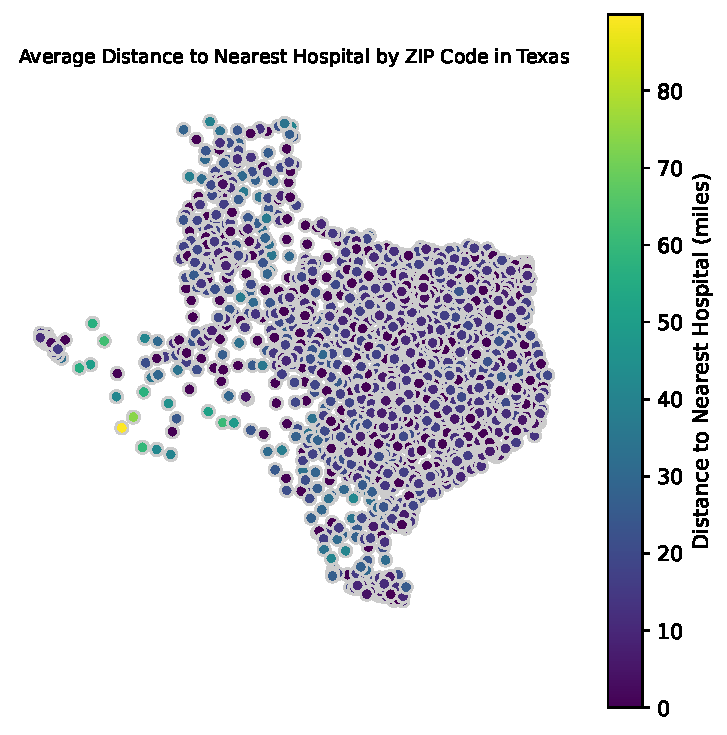
\includegraphics{pset4_template_files/figure-pdf/cell-22-output-1.pdf}

\subsection{Effects of closures on access in Texas (15
pts)}\label{effects-of-closures-on-access-in-texas-15-pts}

\begin{enumerate}
\def\labelenumi{\arabic{enumi}.}
\tightlist
\item
\end{enumerate}

\begin{Shaded}
\begin{Highlighting}[]
\CommentTok{\# Convert ZIP\_CD to string, remove any \textquotesingle{}.0\textquotesingle{} suffix if present}
\NormalTok{closed\_hospitals[}\StringTok{\textquotesingle{}ZIP\_CD\textquotesingle{}}\NormalTok{] }\OperatorTok{=}\NormalTok{ closed\_hospitals[}\StringTok{\textquotesingle{}ZIP\_CD\textquotesingle{}}\NormalTok{].astype(}\BuiltInTok{str}\NormalTok{).}\BuiltInTok{str}\NormalTok{.replace(}\VerbatimStringTok{r\textquotesingle{}\textbackslash{}.0$\textquotesingle{}}\NormalTok{, }\StringTok{\textquotesingle{}\textquotesingle{}}\NormalTok{, regex}\OperatorTok{=}\VariableTok{True}\NormalTok{).}\BuiltInTok{str}\NormalTok{.zfill(}\DecValTok{5}\NormalTok{)}

\CommentTok{\# Filter the closures data based on known Texas ZIP code prefixes)}
\NormalTok{texas\_closures }\OperatorTok{=}\NormalTok{ closed\_hospitals[closed\_hospitals[}\StringTok{\textquotesingle{}ZIP\_CD\textquotesingle{}}\NormalTok{].}\BuiltInTok{str}\NormalTok{.startswith((}\StringTok{\textquotesingle{}75\textquotesingle{}}\NormalTok{, }\StringTok{\textquotesingle{}76\textquotesingle{}}\NormalTok{, }\StringTok{\textquotesingle{}77\textquotesingle{}}\NormalTok{, }\StringTok{\textquotesingle{}78\textquotesingle{}}\NormalTok{, }\StringTok{\textquotesingle{}79\textquotesingle{}}\NormalTok{))]}
\CommentTok{\# Group by ZIP code and count closures}
\NormalTok{closures\_by\_zipcode }\OperatorTok{=}\NormalTok{ texas\_closures.groupby(}\StringTok{\textquotesingle{}ZIP\_CD\textquotesingle{}}\NormalTok{).size().reset\_index(name}\OperatorTok{=}\StringTok{\textquotesingle{}Closure\_Count\textquotesingle{}}\NormalTok{)}

\CommentTok{\# Display the table of closures by ZIP code}
\BuiltInTok{print}\NormalTok{(}\StringTok{"Table of Hospital Closures by ZIP Code in Texas (2016{-}2019):"}\NormalTok{)}
\BuiltInTok{print}\NormalTok{(closures\_by\_zipcode)}

\CommentTok{\# Optionally display the top affected ZIP codes for brevity}
\BuiltInTok{print}\NormalTok{(}\StringTok{"Top Affected ZIP Codes by Hospital Closures:"}\NormalTok{)}
\BuiltInTok{print}\NormalTok{(closures\_by\_zipcode.sort\_values(by}\OperatorTok{=}\StringTok{\textquotesingle{}Closure\_Count\textquotesingle{}}\NormalTok{, ascending}\OperatorTok{=}\VariableTok{False}\NormalTok{).head(}\DecValTok{10}\NormalTok{))}
\end{Highlighting}
\end{Shaded}

\begin{verbatim}
Table of Hospital Closures by ZIP Code in Texas (2016-2019):
   ZIP_CD  Closure_Count
0   75042              1
1   75051              1
2   75087              1
3   75140              1
4   75231              1
5   75235              1
6   75390              1
7   75601              1
8   75662              1
9   75835              1
10  75862              1
11  76502              1
12  76520              1
13  76531              1
14  76645              1
15  77035              1
16  77054              1
17  77065              1
18  77429              1
19  77479              1
20  77598              1
21  78017              1
22  78061              1
23  78336              1
24  78613              1
25  78734              1
26  78834              1
27  79520              1
28  79529              1
29  79553              1
30  79735              1
31  79761              1
32  79902              1
Top Affected ZIP Codes by Hospital Closures:
   ZIP_CD  Closure_Count
0   75042              1
17  77065              1
31  79761              1
30  79735              1
29  79553              1
28  79529              1
27  79520              1
26  78834              1
25  78734              1
24  78613              1
\end{verbatim}

\begin{enumerate}
\def\labelenumi{\arabic{enumi}.}
\setcounter{enumi}{1}
\tightlist
\item
\end{enumerate}

\begin{Shaded}
\begin{Highlighting}[]
\CommentTok{\# Load Texas ZIP codes shapefile and hospital closures data}
\NormalTok{shapefile\_path }\OperatorTok{=} \StringTok{"/Users/attaullah/Documents/problem{-}set{-}4{-}atta/gz\_2010\_us\_860\_00\_500k/gz\_2010\_us\_860\_00\_500k.shp"}  \CommentTok{\# Adjust the path}
\NormalTok{zip\_gdf }\OperatorTok{=}\NormalTok{ gpd.read\_file(shapefile\_path)}

\CommentTok{\# Define Texas ZIP code prefixes and filter the data}
\NormalTok{texas\_zip\_prefixes }\OperatorTok{=}\NormalTok{ [}\StringTok{"75"}\NormalTok{, }\StringTok{"76"}\NormalTok{, }\StringTok{"77"}\NormalTok{, }\StringTok{"78"}\NormalTok{, }\StringTok{"79"}\NormalTok{]}
\NormalTok{zip\_gdf[}\StringTok{"ZCTA5"}\NormalTok{] }\OperatorTok{=}\NormalTok{ zip\_gdf[}\StringTok{"ZCTA5"}\NormalTok{].astype(}\BuiltInTok{str}\NormalTok{)}
\NormalTok{texas\_zip\_gdf }\OperatorTok{=}\NormalTok{ zip\_gdf[zip\_gdf[}\StringTok{"ZCTA5"}\NormalTok{].}\BuiltInTok{str}\NormalTok{.startswith(}\BuiltInTok{tuple}\NormalTok{(texas\_zip\_prefixes))]}

\CommentTok{\# Merge Texas ZIP codes with closure data}
\NormalTok{closures\_by\_zipcode[}\StringTok{\textquotesingle{}ZIP\_CD\textquotesingle{}}\NormalTok{] }\OperatorTok{=}\NormalTok{ closures\_by\_zipcode[}\StringTok{\textquotesingle{}ZIP\_CD\textquotesingle{}}\NormalTok{].astype(}\BuiltInTok{str}\NormalTok{).}\BuiltInTok{str}\NormalTok{.zfill(}\DecValTok{5}\NormalTok{)}
\NormalTok{texas\_closure\_geo }\OperatorTok{=}\NormalTok{ texas\_zip\_gdf.merge(closures\_by\_zipcode, left\_on}\OperatorTok{=}\StringTok{"ZCTA5"}\NormalTok{, right\_on}\OperatorTok{=}\StringTok{"ZIP\_CD"}\NormalTok{, how}\OperatorTok{=}\StringTok{"left"}\NormalTok{)}
\NormalTok{texas\_closure\_geo[}\StringTok{\textquotesingle{}Closure\_Count\textquotesingle{}}\NormalTok{] }\OperatorTok{=}\NormalTok{ texas\_closure\_geo[}\StringTok{\textquotesingle{}Closure\_Count\textquotesingle{}}\NormalTok{].fillna(}\DecValTok{0}\NormalTok{)}
\CommentTok{\# Plot the map}
\NormalTok{fig, ax }\OperatorTok{=}\NormalTok{ plt.subplots(}\DecValTok{1}\NormalTok{, }\DecValTok{1}\NormalTok{, figsize}\OperatorTok{=}\NormalTok{(}\DecValTok{7}\NormalTok{, }\DecValTok{5}\NormalTok{))}
\NormalTok{texas\_closure\_geo.plot(}
\NormalTok{    column}\OperatorTok{=}\StringTok{\textquotesingle{}Closure\_Count\textquotesingle{}}\NormalTok{,}
\NormalTok{    cmap}\OperatorTok{=}\StringTok{\textquotesingle{}OrRd\textquotesingle{}}\NormalTok{,}
\NormalTok{    linewidth}\OperatorTok{=}\FloatTok{0.8}\NormalTok{,}
\NormalTok{    ax}\OperatorTok{=}\NormalTok{ax,}
\NormalTok{    edgecolor}\OperatorTok{=}\StringTok{\textquotesingle{}0.8\textquotesingle{}}\NormalTok{,}
\NormalTok{    legend}\OperatorTok{=}\VariableTok{True}
\NormalTok{)}
\NormalTok{ax.set\_title(}\StringTok{"Texas ZIP Codes Directly Affected by Hospital Closures (2016{-}2019)"}\NormalTok{)}
\NormalTok{ax.set\_axis\_off()}
\NormalTok{plt.show()}
\end{Highlighting}
\end{Shaded}

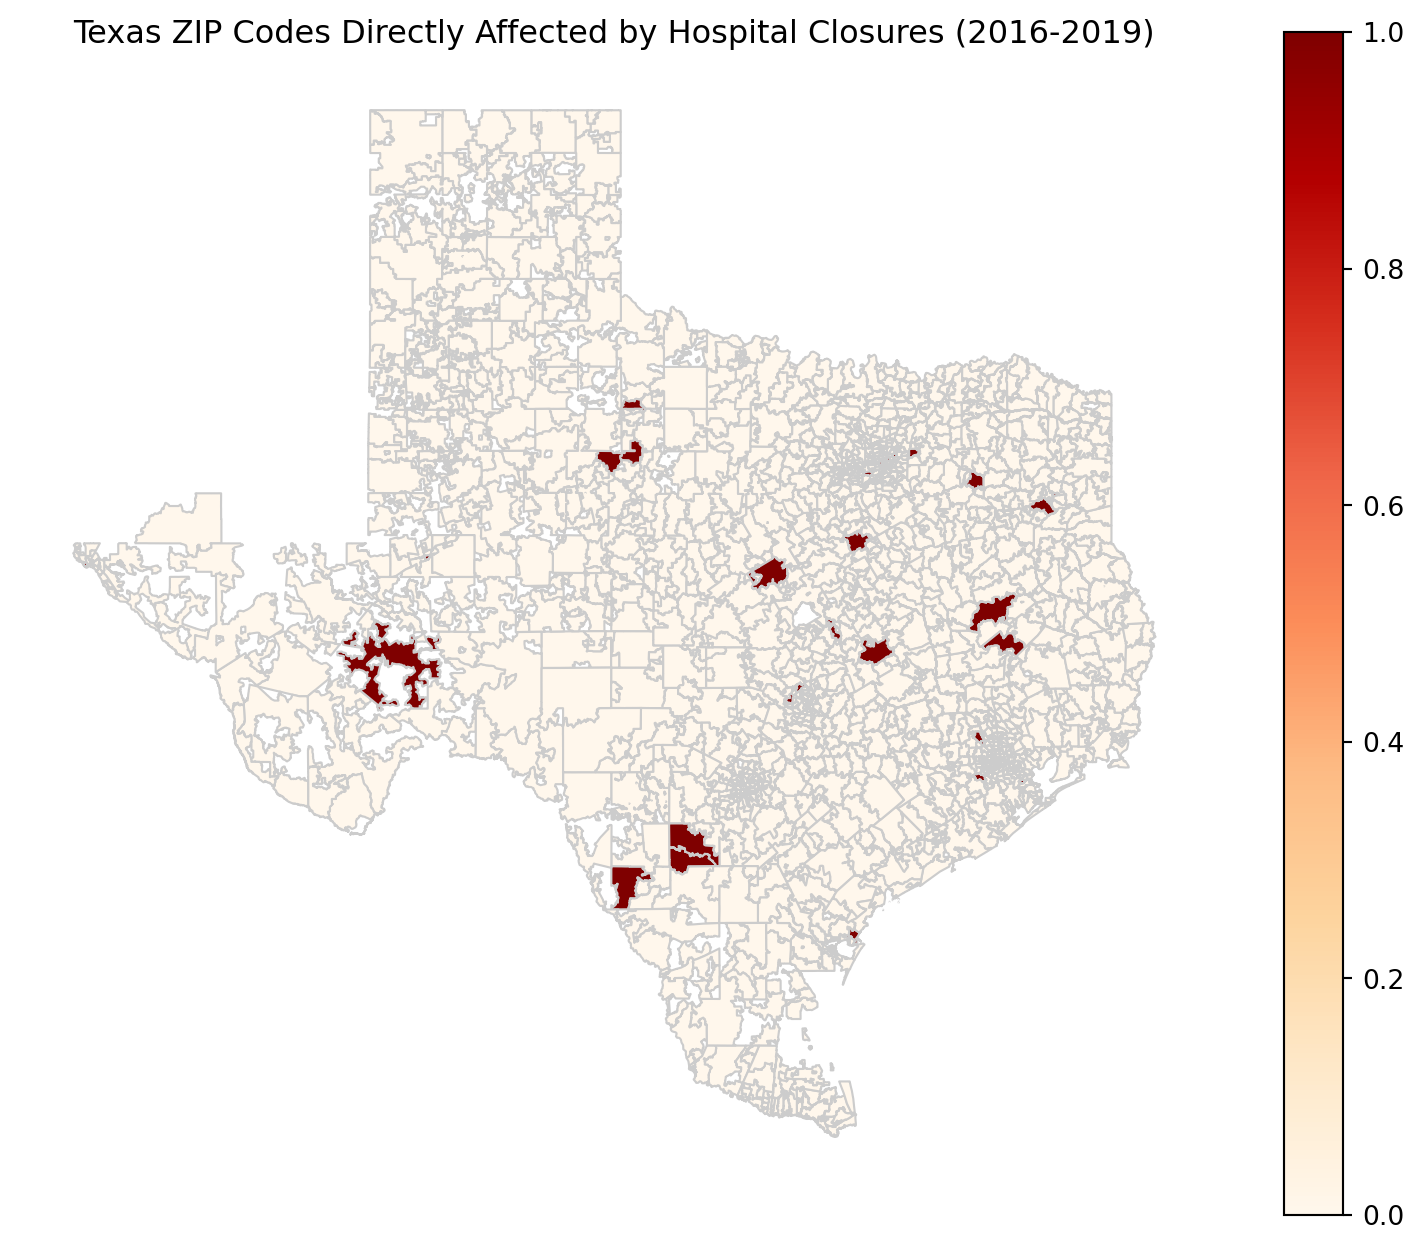
\includegraphics{pset4_template_files/figure-pdf/cell-24-output-1.pdf}

\begin{enumerate}
\def\labelenumi{\arabic{enumi}.}
\setcounter{enumi}{2}
\tightlist
\item
\end{enumerate}

\begin{Shaded}
\begin{Highlighting}[]
\CommentTok{\# Re{-}project to a projected CRS for accurate buffering}
\NormalTok{texas\_zip\_gdf }\OperatorTok{=}\NormalTok{ texas\_zip\_gdf.to\_crs(epsg}\OperatorTok{=}\DecValTok{3395}\NormalTok{)}
\NormalTok{directly\_affected\_zips }\OperatorTok{=}\NormalTok{ texas\_closure\_geo[texas\_closure\_geo[}\StringTok{\textquotesingle{}Closure\_Count\textquotesingle{}}\NormalTok{] }\OperatorTok{\textgreater{}} \DecValTok{0}\NormalTok{].to\_crs(epsg}\OperatorTok{=}\DecValTok{3395}\NormalTok{)}

\CommentTok{\# Step 1: Create a 10{-}mile buffer around directly affected ZIP codes (10 miles ≈ 16093.4 meters)}
\NormalTok{directly\_affected\_zips[}\StringTok{\textquotesingle{}buffer\textquotesingle{}}\NormalTok{] }\OperatorTok{=}\NormalTok{ directly\_affected\_zips.geometry.}\BuiltInTok{buffer}\NormalTok{(}\FloatTok{16093.4}\NormalTok{)  }\CommentTok{\# Buffer in meters}

\CommentTok{\# Step 2: Convert buffered areas to a new GeoDataFrame}
\NormalTok{buffered\_zips }\OperatorTok{=}\NormalTok{ gpd.GeoDataFrame(directly\_affected\_zips[[}\StringTok{\textquotesingle{}ZIP\_CD\textquotesingle{}}\NormalTok{, }\StringTok{\textquotesingle{}buffer\textquotesingle{}}\NormalTok{]], geometry}\OperatorTok{=}\StringTok{\textquotesingle{}buffer\textquotesingle{}}\NormalTok{, crs}\OperatorTok{=}\NormalTok{directly\_affected\_zips.crs)}

\CommentTok{\# Step 3: Perform spatial join }
\NormalTok{indirectly\_affected\_zips }\OperatorTok{=}\NormalTok{ gpd.sjoin(texas\_zip\_gdf, buffered\_zips, how}\OperatorTok{=}\StringTok{\textquotesingle{}inner\textquotesingle{}}\NormalTok{, predicate}\OperatorTok{=}\StringTok{\textquotesingle{}intersects\textquotesingle{}}\NormalTok{)}

\CommentTok{\# Step 4: Count unique ZIP codes in the indirectly affected set}
\NormalTok{indirectly\_affected\_count }\OperatorTok{=}\NormalTok{ indirectly\_affected\_zips[}\StringTok{\textquotesingle{}ZIP\_CD\textquotesingle{}}\NormalTok{].nunique()}
\BuiltInTok{print}\NormalTok{(}\StringTok{"Number of indirectly affected ZIP codes:"}\NormalTok{, indirectly\_affected\_count)}
\end{Highlighting}
\end{Shaded}

\begin{verbatim}
Number of indirectly affected ZIP codes: 33
\end{verbatim}

\begin{enumerate}
\def\labelenumi{\arabic{enumi}.}
\setcounter{enumi}{3}
\tightlist
\item
\end{enumerate}

\begin{Shaded}
\begin{Highlighting}[]
\CommentTok{\# Step 1: Re{-}project data for accuracy (if not already done)}
\NormalTok{texas\_zip\_gdf }\OperatorTok{=}\NormalTok{ texas\_zip\_gdf.to\_crs(epsg}\OperatorTok{=}\DecValTok{3395}\NormalTok{)}
\NormalTok{directly\_affected\_zips }\OperatorTok{=}\NormalTok{ texas\_closure\_geo[texas\_closure\_geo[}\StringTok{\textquotesingle{}Closure\_Count\textquotesingle{}}\NormalTok{] }\OperatorTok{\textgreater{}} \DecValTok{0}\NormalTok{].to\_crs(epsg}\OperatorTok{=}\DecValTok{3395}\NormalTok{)}

\CommentTok{\# Step 2: Create a 10{-}mile buffer around directly affected ZIP codes}
\NormalTok{directly\_affected\_zips[}\StringTok{\textquotesingle{}buffer\textquotesingle{}}\NormalTok{] }\OperatorTok{=}\NormalTok{ directly\_affected\_zips.geometry.}\BuiltInTok{buffer}\NormalTok{(}\FloatTok{16093.4}\NormalTok{)  }\CommentTok{\# Buffer in meters}
\NormalTok{buffered\_zips }\OperatorTok{=}\NormalTok{ gpd.GeoDataFrame(directly\_affected\_zips[[}\StringTok{\textquotesingle{}ZCTA5\textquotesingle{}}\NormalTok{, }\StringTok{\textquotesingle{}buffer\textquotesingle{}}\NormalTok{]], geometry}\OperatorTok{=}\StringTok{\textquotesingle{}buffer\textquotesingle{}}\NormalTok{, crs}\OperatorTok{=}\NormalTok{directly\_affected\_zips.crs)}

\CommentTok{\# Step 3: Identify indirectly affected ZIP codes}
\NormalTok{indirectly\_affected\_zips }\OperatorTok{=}\NormalTok{ gpd.sjoin(texas\_zip\_gdf, buffered\_zips, how}\OperatorTok{=}\StringTok{\textquotesingle{}inner\textquotesingle{}}\NormalTok{, predicate}\OperatorTok{=}\StringTok{\textquotesingle{}intersects\textquotesingle{}}\NormalTok{)}
\NormalTok{indirectly\_affected\_zip\_codes }\OperatorTok{=}\NormalTok{ indirectly\_affected\_zips[}\StringTok{\textquotesingle{}ZCTA5\_left\textquotesingle{}}\NormalTok{].unique()  }\CommentTok{\# Use \textquotesingle{}ZCTA5\_left\textquotesingle{} from join result}

\CommentTok{\# Step 4: Classify ZIP codes into categories}
\NormalTok{texas\_zip\_gdf[}\StringTok{\textquotesingle{}category\textquotesingle{}}\NormalTok{] }\OperatorTok{=} \StringTok{\textquotesingle{}Not Affected\textquotesingle{}}
\NormalTok{texas\_zip\_gdf.loc[texas\_zip\_gdf[}\StringTok{\textquotesingle{}ZCTA5\textquotesingle{}}\NormalTok{].isin(directly\_affected\_zips[}\StringTok{\textquotesingle{}ZCTA5\textquotesingle{}}\NormalTok{]), }\StringTok{\textquotesingle{}category\textquotesingle{}}\NormalTok{] }\OperatorTok{=} \StringTok{\textquotesingle{}Directly Affected\textquotesingle{}}
\NormalTok{texas\_zip\_gdf.loc[(texas\_zip\_gdf[}\StringTok{\textquotesingle{}ZCTA5\textquotesingle{}}\NormalTok{].isin(indirectly\_affected\_zip\_codes)) }\OperatorTok{\&} 
\NormalTok{                  (}\OperatorTok{\textasciitilde{}}\NormalTok{texas\_zip\_gdf[}\StringTok{\textquotesingle{}ZCTA5\textquotesingle{}}\NormalTok{].isin(directly\_affected\_zips[}\StringTok{\textquotesingle{}ZCTA5\textquotesingle{}}\NormalTok{])), }\StringTok{\textquotesingle{}category\textquotesingle{}}\NormalTok{] }\OperatorTok{=} \StringTok{\textquotesingle{}Indirectly Affected\textquotesingle{}}

\CommentTok{\# Step 5: Plot the choropleth}
\NormalTok{fig, ax }\OperatorTok{=}\NormalTok{ plt.subplots(}\DecValTok{1}\NormalTok{, }\DecValTok{1}\NormalTok{, figsize}\OperatorTok{=}\NormalTok{(}\DecValTok{7}\NormalTok{, }\DecValTok{5}\NormalTok{))}
\NormalTok{category\_colors }\OperatorTok{=}\NormalTok{ \{}\StringTok{\textquotesingle{}Not Affected\textquotesingle{}}\NormalTok{: }\StringTok{\textquotesingle{}lightgrey\textquotesingle{}}\NormalTok{, }\StringTok{\textquotesingle{}Directly Affected\textquotesingle{}}\NormalTok{: }\StringTok{\textquotesingle{}red\textquotesingle{}}\NormalTok{, }\StringTok{\textquotesingle{}Indirectly Affected\textquotesingle{}}\NormalTok{: }\StringTok{\textquotesingle{}orange\textquotesingle{}}\NormalTok{\}}
\NormalTok{texas\_zip\_gdf.plot(column}\OperatorTok{=}\StringTok{\textquotesingle{}category\textquotesingle{}}\NormalTok{, categorical}\OperatorTok{=}\VariableTok{True}\NormalTok{, }
\NormalTok{                   legend}\OperatorTok{=}\VariableTok{True}\NormalTok{, color}\OperatorTok{=}\NormalTok{[category\_colors.get(x) }\ControlFlowTok{for}\NormalTok{ x }\KeywordTok{in}\NormalTok{ texas\_zip\_gdf[}\StringTok{\textquotesingle{}category\textquotesingle{}}\NormalTok{]],}
\NormalTok{                   legend\_kwds}\OperatorTok{=}\NormalTok{\{}\StringTok{\textquotesingle{}title\textquotesingle{}}\NormalTok{: }\StringTok{"Impact Category"}\NormalTok{\}, ax}\OperatorTok{=}\NormalTok{ax, edgecolor}\OperatorTok{=}\StringTok{\textquotesingle{}black\textquotesingle{}}\NormalTok{)}

\CommentTok{\# Adding a title and displaying the plot}
\NormalTok{plt.title(}\StringTok{"Texas ZIP Codes Categorized by Impact of Hospital Closures (2016{-}2019)"}\NormalTok{)}
\NormalTok{plt.axis(}\StringTok{\textquotesingle{}off\textquotesingle{}}\NormalTok{)  }\CommentTok{\# Hide axis for a cleaner look}
\NormalTok{plt.show()}
\end{Highlighting}
\end{Shaded}

\includegraphics{pset4_template_files/figure-pdf/cell-26-output-1.pdf}

\subsection{Reflecting on the exercise (10
pts)}\label{reflecting-on-the-exercise-10-pts}

\begin{enumerate}
\def\labelenumi{\arabic{enumi}.}
\tightlist
\item
\end{enumerate}

\begin{itemize}
\tightlist
\item
  The first-pass method risks misidentifying closures because it doesn't
  account for temporary closures, facility mergers, or changes in
  hospital IDs. This can lead to over- or under-counting affected areas.
  To improve, we could:
\item
  Cross-reference closures with state and local health department data
  to verify permanent status.
\item
  Track hospital utilization trends over time to differentiate between
  closures and service reductions.
\item
  Use multiple years of data to confirm if facilities remain closed
  rather than reopening under new identifiers.
\item
  Integrate local news reports and community health resources to
  validate closures.
\item
  These steps could make the identification process more accurate and
  reduce misclassification.
\end{itemize}

\begin{enumerate}
\def\labelenumi{\arabic{enumi}.}
\setcounter{enumi}{1}
\tightlist
\item
\end{enumerate}

\begin{itemize}
\tightlist
\item
  The current approach, identifying affected ZIP codes based on a
  10-mile radius around closures, provides a rough estimate but doesn't
  fully capture changes in access. Here are some ways to improve:
\item
  Travel Time Analysis: Use drive time rather than straight-line
  distance, as actual access depends on road networks, traffic, and
  transportation options.
\item
  Population Density and Demand: Factor in population density and local
  demand to assess how many people are impacted within each affected ZIP
  code.
\item
  Alternative Facilities: Account for nearby hospitals or healthcare
  facilities that could serve as substitutes, providing a more realistic
  measure of lost access.
\item
  Demographic and Socioeconomic Factors: Include variables like age,
  income, and car ownership to reflect differences in accessibility and
  reliance on local hospitals across communities.
\item
  These adjustments could give a more accurate picture of how hospital
  closures impact healthcare access at the ZIP-code level.
\end{itemize}




\end{document}
